\documentclass[12pt]{article}

\usepackage{blindtext} % Package to generate dummy text throughout this template 

% writing
\usepackage[utf8]{inputenc}
\usepackage{amssymb, amsthm}
\usepackage{algorithm}
\usepackage[noend]{algpseudocode}
\linespread{1.5}
\usepackage[margin = 1in]{geometry}
\usepackage{microtype} % Slightly tweak font spacing for aesthetics
\usepackage[english]{babel} % Language hyphenation and typographical rules

% tikz
\usepackage{tikz}
\usepackage{pgfplots}
\usepackage{pgfplotstable}
\pgfplotsset{compat=1.13}

% fig
\usepackage{natbib}
\usepackage{graphicx}
\usepackage{float}
\usepackage{wrapfig}
\usepackage{multicol}

% misc
\usepackage{nomencl}
\usepackage[titletoc, page]{appendix}
\usepackage{multirow}

% caption features
\usepackage{caption}
\usepackage{subcaption}
\usepackage{setspace}
\captionsetup{font={small, stretch=1.25}}
\let\Algorithm\algorithm
\renewcommand\algorithm[1][]{\Algorithm[#1]\setstretch{1.25}}

% ref
\usepackage[pdfpagelabels]{hyperref}
\usepackage{url}
\hypersetup{
    colorlinks=true,
    linkcolor=black,      
    urlcolor=black,
    citecolor=black
}
\usepackage{cleveref}
\crefformat{section}{\S#2#1#3}
\crefformat{subsection}{\S#2#1#3}
\crefformat{subsubsection}{\S#2#1#3}

\usepackage{amsmath}    % conflicts with cleveref

\setlength{\parindent}{2em}
%\setlength{\parskip}{1.5em}
\graphicspath{ {images/} }

% nomenclature specs
\makenomenclature
\setlength{\nomitemsep}{-\parsep}
\renewcommand{\nomname}{List of Functions, Symbols \& Terms}
%% This code creates the groups
% -----------------------------------------
\usepackage{etoolbox}
\renewcommand{\nomgroup}[1]{%
    \item[\bfseries
    \ifstrequal{#1}{T}{Terms}{%
        \ifstrequal{#1}{S}{Symbols}{%
            \ifstrequal{#1}{F}{Functions}{}}%
    }]}
% -----------------------------------------

\newtheorem{mydef}{Definition}
\newcommand{\vect}[1]{\mathbf{#1}}  % vector
\newcommand{\matr}[1]{\mathbf{#1}}  % matrix
\newcommand{\tens}[1]{\mathbf{#1}}  % tensor
\newcommand{\mean}[1]{\overline{#1}}    % mean overline

\title{Report: Solving the Avicaching Problem Faster and Better}
\author{Anmol Kabra, Yexiang Xue \& Carla Gomes}
\date{Summer 2017}

\begin{document}
    \pagenumbering{roman}
    \begin{titlepage}
        \maketitle
        \thispagestyle{empty}
    \end{titlepage}
    
    % nomenclature
    \mbox{}
    % symbols
    \nomenclature[S]{$J$}{Number of locations in the dataset}
    \nomenclature[S]{$T$}{Number of time units for which data is available}
    \nomenclature[S]{$n_F$}{Number of features in the dataset $\matr{F}$ (length of $\matr{F}[v][u]$)}
    
    % functions
    \nomenclature[F]{softmax($\cdot$)}{Defined as softmax($z_i$) = $\frac{\exp(z_i)}{\sum_{i} \exp(z_i)}$}
    \nomenclature[F]{reLU($\cdot$)}{Rectified Linear Unit; defined as reLU($z$) = max(0, $z$)}
    \nomenclature[F]{batch-multiply($\cdot$)}{Operates on $m \times n \times p$ and $m \times p \times q$ tensors to give a $m \times n \times q$ tensor.}
    
    % terms
    \nomenclature[T]{Epoch}{One training/testing period; iteration}
    \nomenclature[T]{CPU ``set''}{\textit{All} operations done on the CPU}
    \nomenclature[T]{GPU ``set''}{\textit{Only Matrix/Tensor} operations done on the GPU, rest on the CPU}
    \nomenclature[T]{LP}{Linear Programming}
    \nomenclature[T]{LP Standard Format}{Arrangement of objective function and constraints operated on by library LP solvers - minimize [$\vect{c}^T \vect{x}$]; subject to [$\matr{A} \vect{x} \leq \vect{b}, \, x_i \geq 0$]}
    \nomenclature[T]{Tensor}{Multi-dimensional (usually more than 2 dimensions) array}
    \printnomenclature[1.5in]
    \cleardoublepage
    
    \tableofcontents
    \listoftables
    \listoffigures
    \cleardoublepage
    \pagenumbering{arabic}
    % main body
    \section{Introduction} \label{sec:Introduction}
    Optimizing predictive models on datasets obtained from citizen-science projects can be computationally expensive as these datasets grow in size with time. Consequently, models based on multi-layered neural networks, Integer Programming and other optimization routines can prove increasingly difficult as the number of parameters increase, despite using the faster Central Processing Units (CPUs) in the market. Incidentally, it becomes difficult for citizen-science projects to scale if the organizers use CPUs to run optimization models. However, Graphical Processing Units (GPUs), which offer multiple cores to parallelize computation, can outperform CPUs in computing such predictive models if these models heavily rely on large-scale matrix multiplications. By using GPUs over CPUs to accelerate computation on a citizen-science project, the model could achieve better optimization in less time, enabling the project to scale.
    
    \subsection{Avicaching}
    Part of the eBird project, which aims to ``maximize the utility and accessibility of the vast numbers of bird observations made each year by recreational and professional bird watchers'' [cite website], Avicaching is a incentive-driven game trying to homogenize the spatial distribution of citizens' (agents') observations \cite{Xue2016Avi1}. Since the dataset of agents' observations in eBird is geographically heterogeneous (concentrated in some places like cities and sparse in others), Avicaching homogenizes the observation set by placing rewards and attracting agents at under-sampled locations \cite{Xue2016Avi1}. For the agents, collecting rewards increases their 'utility' (excitement or fun), while for the organizers, a more homogeneous observation dataset means better sampling and validates the models' applicability. 
    
    To accomplish this task of specifying rewards at different locations based on the historical records of observations, Avicaching would learn how agents change their behavior when a certain sample of rewards were applied to the set of locations, and then distribute a newer set of rewards across the locations based on those learned parameters \cite{Xue2016Avi2}. This requirement naturally translates into a predictive optimization problem, which is implemented using multi-layered neural networks and linear programming.
    
    \subsection{Important Questions}
    Although the previously devised solutions to Avicaching were conceptually effective \cite{Xue2016Avi1}\cite{Xue2016Avi2}, using CPUs to solve Mixed Integer Programming and shallow neural networks made the solutions impractical to scale. Solving the problems faster would have also allowed organizers to find better results (more optimized). These concerns, which form the pivot for our research, are concisely described in next sections.
    
    \subsubsection{Solving Faster} \label{sec:Important Questions - Solving Faster}
    We were interested in using GPUs, with their growing capability to accelerate problems based on large matrix and tensor operations, to run our optimization models. Newer generation NVIDIA GPUs equipped with thousands of CUDA (NVIDIA's parallel computing API) cores \cite{NVIDIA} could have empowered Avicaching's organizers to scale the game, if the game was computed using simple arithmetic operations on tensors, rather than using conditional logic (why? - reasoned in \cref{sec:Computation Using GPUs}). Since even the faster CPUs - in the range of Intel Core i7 chipsets - are sequential in processing and do not provide as comparable parallel processing as GPUs do, we believed to solve the problem much faster using GPUs. \textbf{But how much faster?}
    
    \subsubsection{Better Results} \label{sec:Important Questions - Better Results}
    The previous model, for learning the parameters in agents' change of behavior on a fixed set of rewards, delivered predictions that differed 26\% from Ground Truth \cite[// todo]{Xue2016Avi2}. This model was then used to distribute a new set of rewards in a budget. If we could get closer to the Ground Truth, i.e., better learn the parameters for the change, we could distribute a new set of rewards based on superior prediction. Since the organizers need the \textit{best} distribution of rewards (our motive in this research too), we would need a set of learned parameters that is closer to the Ground Truth (in terms of Normalized Mean Squared Error \cite[// todo]{Xue2016Avi2}). In a gist, we aimed to \textbf{learn the parameters more suitably}, and find the \textbf{best allocation of rewards?}
    
    \subsubsection{Adjusting the Model's Features} \label{sec:Important Questions - Adjusting the Model's Features}
    Once our model starts delivering better results than the previously devised models, one thinks if some characteristics of the model (hyper-parameters such as learning rate) can be changed to get more preferable results (though one could also build a better model too). While a goal of ``getting better results'' may seem like an unending strife, there is a trade-off with practicality as these adjustments take time and computation power to test - and we didn't have unlimited resources. Therefore, we asked if one could \textbf{reasonably adjust hyper-parameters to improve performance and optimization.} By ``reasonable adjustments'' we mean changes that improve performance by more than [// todo]5 times using comparable resources.
    
    \subsection{Computation Using GPUs} \label{sec:Computation Using GPUs}
    // todo
    
    \section{Problem Formulation} \label{sec:Problem Formulation}
    Since NVIDIA General Purpose GPUs enable faster computation on tensors, accelerated through CUDA and cuDNN (CUDA Deep Neural Network library) \cite{NVIDIA}, both the Identification and the Pricing Problem (see \cref{sec:Identification Problem} and \cref{sec:Pricing Problem}) were formulated as tensor-based 3-layered and 2-layered neural networks respectively using the PyTorch library \cite{PTDocs}.
    
    \subsection{Identification Problem} \label{sec:Identification Problem}
    As discussed in \cref{sec:Introduction}, the model should learn parameters that caused the change in agents' behavior when a certain set of rewards was applied to locations in the experiment region. Learning those parameters will help us understand how agents behave with a fixed reward distribution, and will enable organizers to redistribute rewards based on that behavior.
    
    Specifically, given datasets $\vect{y_t}$ and $\vect{x_t}$ of agents' visit densities, with and without the rewards $\vect{r_t}$, we want to find weights $\matr{w_1}$ and $\matr{w_2}$ that caused the change from $\vect{x_t}$ to $\vect{y_t}$, factoring in possible influence from environmental factors $\matr{f}$ and distances between locations $\matr{D}$. Although the original model proposed to learn a single set of weights $\matr{w}$ \cite{Xue2016Avi2}, our proposed model considers two sets of weights $\matr{w_1}$ and $\matr{w_2}$ as it may theoretically result into higher accuracy and lower loss. Mathematically, the model can be formulated as:
    \begin{equation} \label{eq:iden_problem}
        \begin{aligned}
            & \underset{\matr{w_1}, \matr{w_2}}{\text{minimize}}
            & & Z_I(\matr{w_1}, \matr{w_2}) = \sum_{t} (\omega_t(\vect{y_t} - \matr{P}(\matr{f}, \vect{r_t}; \matr{w_1}, \matr{w_2})\vect{x_t}))^{2}
        \end{aligned}
    \end{equation}
    where $\omega_t$ is a set of weights (not a learnable parameter) at time $t$ capturing penalties relative to the priority of homogenizing different locations at time $t$. In other words, it highlights if the organizer wishes higher homogeneity at one time over another. Elements $p_{u, v}$ of $\matr{P}$ are given as:
    \begin{equation} \label{eq:puv_equation}
    p_{u, v} = \frac{\exp(\matr{w_2} \cdot \text{reLU} (\matr{w_1} \cdot [d_{u, v}, \vect{f_{u}}, r_{u}]))}{\sum_{u'} \exp(\matr{w_2} \cdot \text{reLU} (\matr{w_1} \cdot [d_{u', v}, \vect{f_{u'}}, r_{u'}]))} = \frac{\exp(\Gamma_{u, v})}{\sum_{u'}\exp(\Gamma_{u', v})} = \text{softmax}(\Gamma_{u, v})
    \end{equation}
    To optimize the loss value $Z_I(\matr{w_1}, \matr{w_2})$, the neural network learns the set of weights through multiple epochs of backpropagating the loss using gradient descent. Furthermore, the program processes the dataset before feeding to the network to avoid unnecessary sub-epoch iterations and to promote batch operations on tensors. 
    
    \subsubsection{Structure of Input Dataset for Identifying Weights} \label{sec:Structure of Input Dataset for Identifying Weights}
    \begin{figure}[!htbp]
        \begin{subfigure}{.64\textwidth}
            \centering
            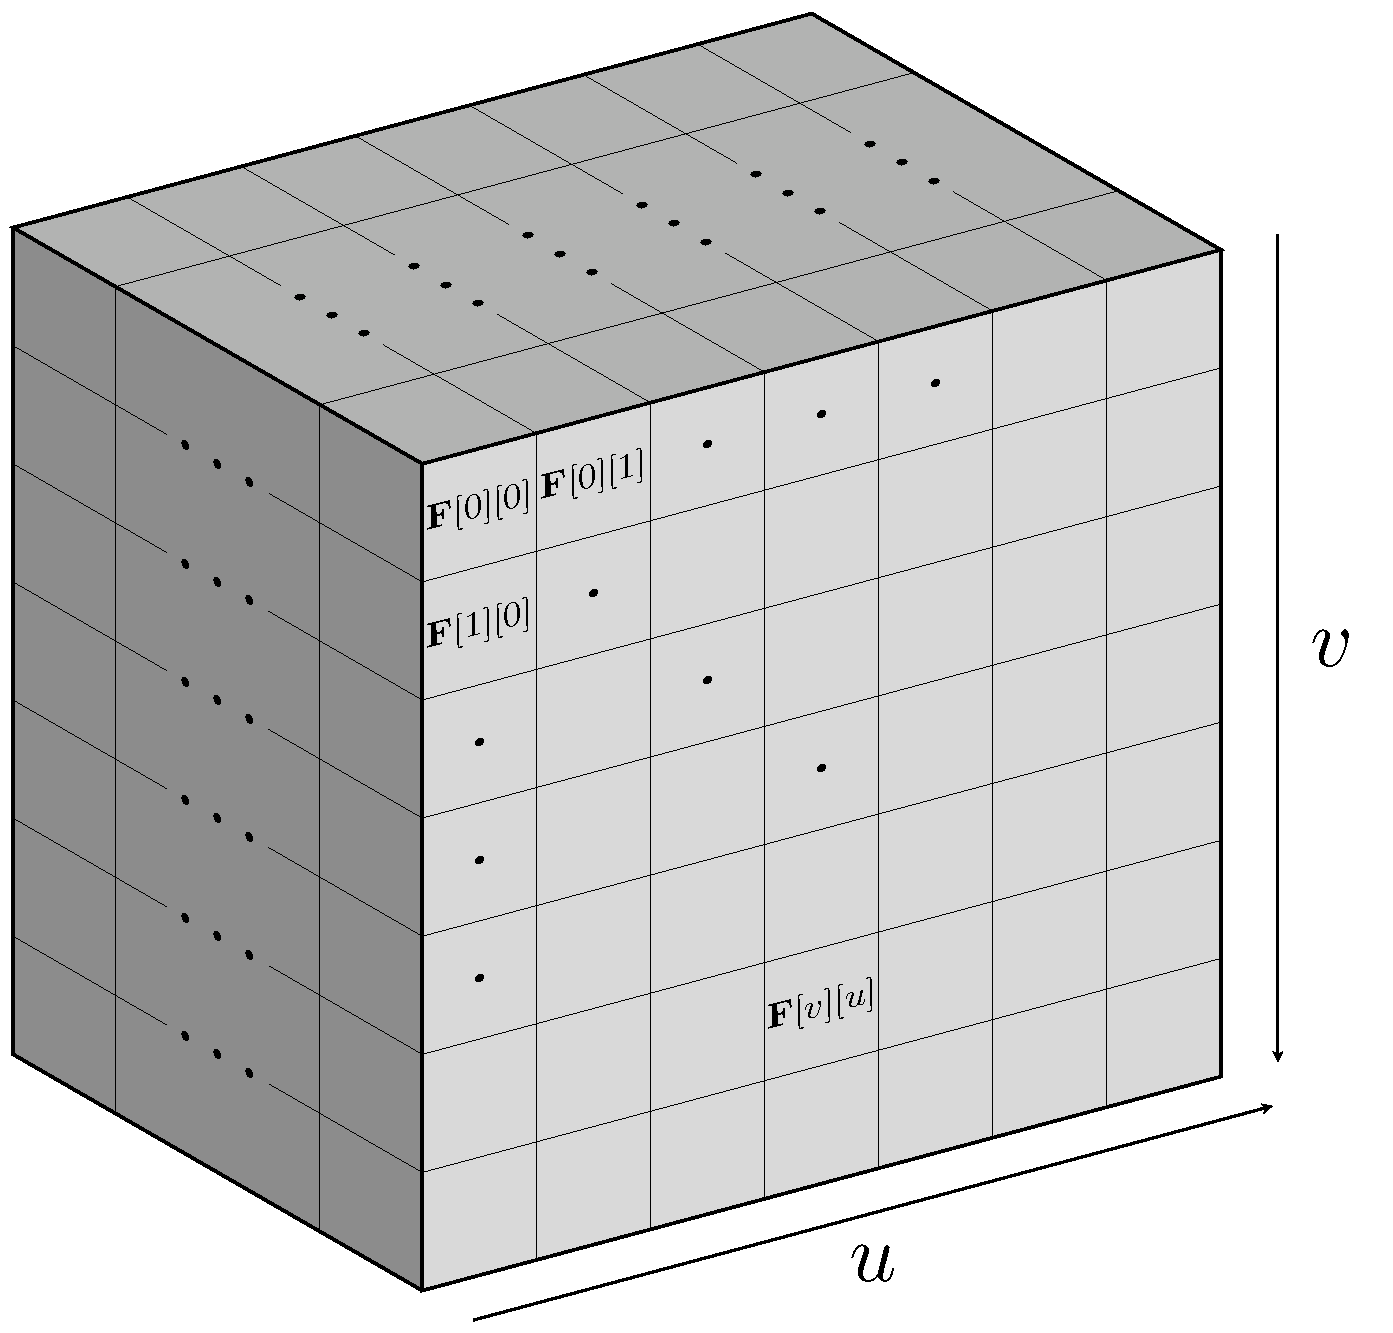
\includegraphics[width=\linewidth]{weights_input_dataset}
            \caption{A Tensor representing the Input Dataset $\tens{F}$}
            \label{fig:A Tensor representing the complete Input Dataset}
        \end{subfigure}
        \begin{subfigure}{.35\textwidth}
            \centering
            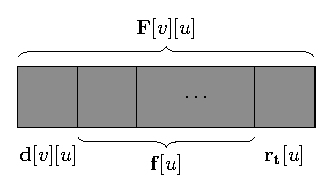
\includegraphics[width=\linewidth]{zoomup_Fuv}
            \caption{Contents of $\tens{F}[v][u]$: This vector (length $n_F$) contains quantified causes for the change in agents' behavior from $\matr{x_t}$ to $\matr{y_t}$}
            \label{fig:Zoomed-in contents of Fvu}
        \end{subfigure}
        \caption{Visual representation of the Input Dataset}
        \label{fig:Visual representation of the Input Dataset}
    \end{figure}
    Since preprocessing the dataset impacts the efficiency of the network, the input dataset, comprising of distance between locations $\matr{D}$, environmental features $\vect{f}$ and given rewards $\vect{r_t}$ (all normalized), is built in a specific manner. Because GPUs are efficient in operating on matrices and tensors, the input dataset is built into a tensor (Figure \ref{fig:A Tensor representing the complete Input Dataset}) such that operations can be performed on batches of slices $\tens{F}[v]$.
    
    Another advantage of building the dataset as a tensor comes with the PyTorch library, which provides convenient handling and transfer of tensors residing on CPUs and GPUs \cite{PTDocs}. Algorithm \ref{alg:Constructing the Input Dataset} describes the steps to construct this dataset.
    \begin{algorithm}
        \caption{Constructing the Input Dataset} \label{alg:Constructing the Input Dataset}
        \begin{algorithmic}[1]
            \Function{Build-Dataset}{$\matr{D}, \matr{f}, \matr{r_t}$}
            \State $\matr{D} \gets \Call{Normalize}{\matr{D}}$\Comment{$\matr{D}[u][v]$ is the distance between locations $u$ and $v$}
            \State $\vect{f} \gets \Call{Normalize}{\mathbf{f}, axis = 0}$\Comment{$\mathbf{f}[u]$ is a vector of env. features at location $u$}
            \State $\vect{r_t} \gets \Call{Normalize}{\vect{r_t}, axis = 0}$\Comment{$\vect{r_t}[u]$ is the reward at location $u$}
            \For{$v = 1, 2, \dots, J$}
                \For{$u = 1, 2, \dots, J$}
                    \State $\tens{F}[v][u] \gets [\matr{D}[v][u], \vect{f}[u], \vect{r_t}[u]]$ \Comment{As depicted in Figure \ref{fig:Zoomed-in contents of Fvu}}
                 \EndFor
            \EndFor
            \State \Return $\matr{F}$
            \EndFunction
        \end{algorithmic}
    \end{algorithm}

    \subsubsection{Minimizing Loss for the Identification Problem} \label{sec:Minimizing Loss for the Identification Problem}
    As shown in Figure \ref{fig:Neural network designed for the Identification Problem}, the neural network is made of 3 fully connected layers - the input layer, the hidden layer with rectified Linear Units (reLU), and the output layer generating the results using the softmax$(\cdot)$ function. The network can also be visualized as a collection of 1-dimensional layers (Figure \ref{fig:Side view of the network}), with the softmax$(\cdot)$ calculated on the collection's output.
    \begin{figure}[!htbp]
        \centering
        \begin{subfigure}{\textwidth}
            \centering
            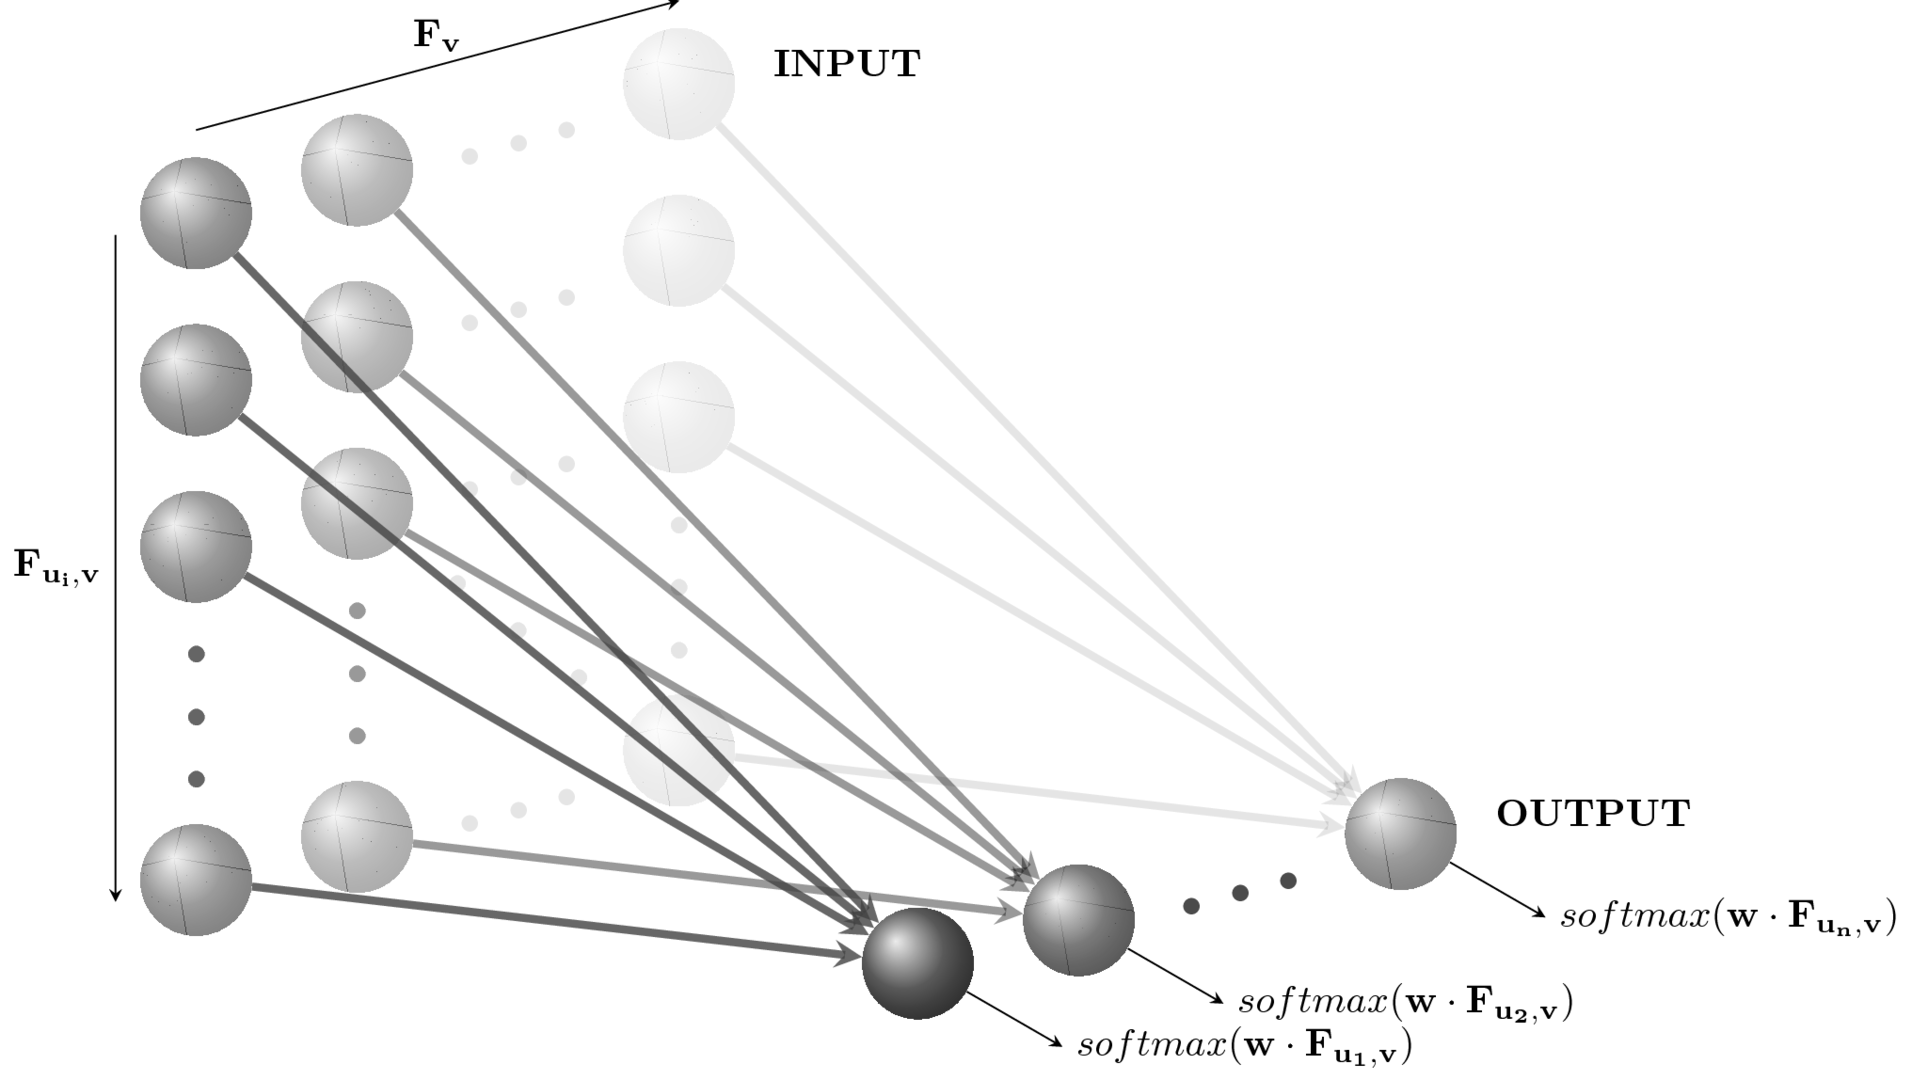
\includegraphics[width=\textwidth]{weights_net}
            \caption{3-dimensional View of the Network Slice, Taking in $\matr{F}[v]$}
            \label{fig:3-dimensional view of the network slice, taking in Fv}
        \end{subfigure}
        \begin{subfigure}{.75\textwidth}
            \centering
            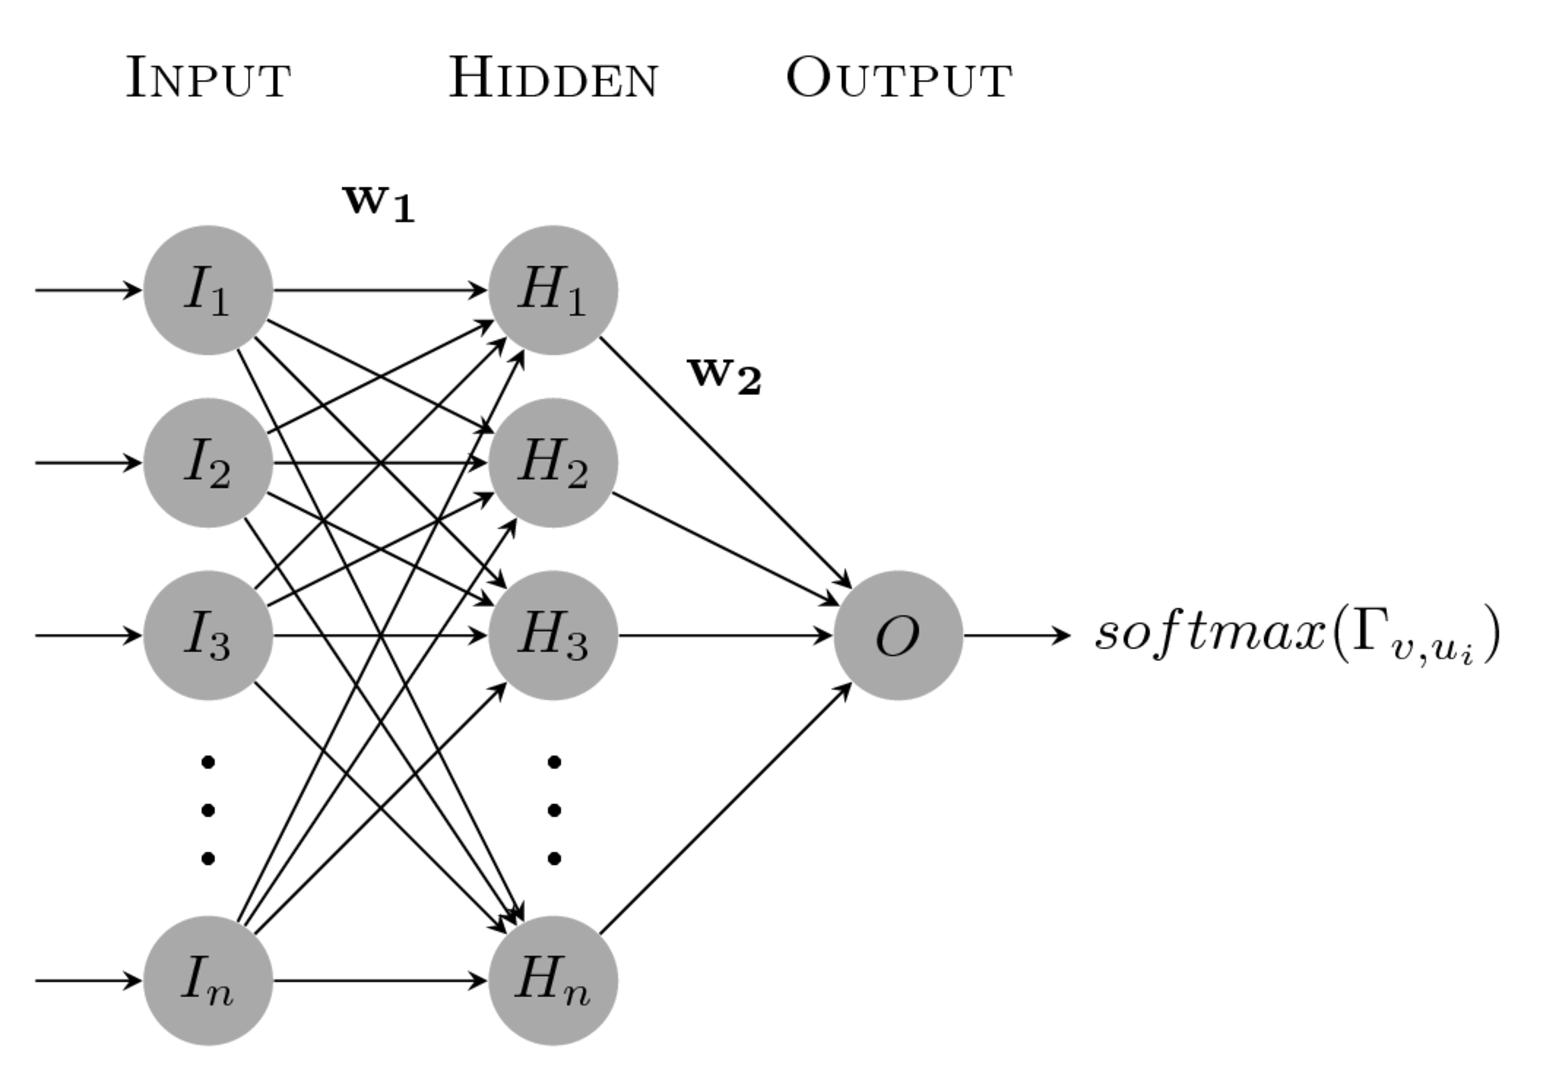
\includegraphics[width=\textwidth]{weights_net_side}
            \caption{Side View of the Network: Output of one such cross-section is $p_{u_i, v}$}
            \label{fig:Side view of the network}
        \end{subfigure}
        \caption{Neural Network Designed for the Identification Problem}
        \label{fig:Neural network designed for the Identification Problem}
    \end{figure}
    It is important to clarify that the network in Figure \ref{fig:3-dimensional view of the network slice, taking in Fv}, which takes in $\matr{F}[v]$ as shown, is a slice of the original network, which takes in the complete tensor $\matr{F}$ and computes the complete result $\matr{P}^{T}$  per iteration of $t$. In other words, the input and the hidden layers are 3-dimensional, and the output layer is 2-dimensional. Since it is difficult to visualize the complete network on paper, slices of the network are depicted in Figure \ref{fig:3-dimensional view of the network slice, taking in Fv}. Algorithm \ref{alg:Algorithm for the Identification Problem} details the steps for learning the parameters $\matr{w_1}$ and $\matr{w_2}$ based on Equations \ref{eq:iden_problem} \& \ref{eq:puv_equation}.
    
    \begin{algorithm}
        \caption{Algorithm for the Identification Problem} \label{alg:Algorithm for the Identification Problem}
        \begin{algorithmic}[1]
            \State $\matr{w_1} \gets \Call{Random}{\;(J,n_F,n_F)\;}$\Comment{$\matr{w_1}$ has dimensions $J \times n_F \times n_F$}
            \State $\matr{w_2} \gets \Call{Random}{\;(J,n_F,1)\;}$\Comment{$\matr{w_2}$ has dimensions $J \times n_F \times 1$}
            \For{$e = 1, 2, \dots, \text{Epochs}$}
                \State $loss \gets 0$
                \For{$t = 1, 2, \dots, T$}
                    \State $\matr{F} \gets \Call{Build-Dataset}{\matr{D}, \matr{f}, \matr{r}[t]}$\Comment{Defined in Algorithm \ref{alg:Constructing the Input Dataset}}
                    \State $\matr{H} \gets  \text{reLU}(\Call{Batch-Multiply}{\matr{F}, \matr{w_1}})$
                    \State $\matr{O} \gets \text{softmax}(\Call{Batch-Multiply}{\matr{H}, \matr{w_2}})$
                    \State $\matr{P} \gets \matr{O}^T$
                    \State $loss \gets loss + (\omega(\matr{y}[t] - \matr{P} \cdot \matr{x}[t]))^2$
                \EndFor
                \State $\Call{Gradient-Descent}{loss, \matr{w_1}, \matr{w_2}}$
                \State $\matr{w_1}, \matr{w_2} \gets \Call{Update-Using-Gradients}{\matr{w_1}, \matr{w_2}}$
                \State $\Call{Log-Info}{e, loss}$
            \EndFor
        \end{algorithmic}
    \end{algorithm}
    
    \subsection{Pricing Problem} \label{sec:Pricing Problem}
    After learning the set of weights $\matr{w_1}$ and $\matr{w_2}$ highlighting the change in agents' behavior to collect observations, the Pricing Problem aims to redistribute rewards to the all locations such that the predicted behavior of agents influenced by the new set of rewards is homogeneous. Thus, given a budget of rewards $\mathcal{R}$, this optimization problem can be expressed as:
    \begin{equation} \label{eq:pricing_problem}
        \begin{aligned}
            & \underset{\vect{r}}{\text{minimize}}
            & & Z_P(\vect{r}) = \frac{1}{n}\lVert \vect{y} - \mean{\vect{y}} \rVert\\
            & \text{subject to}
            & & \vect{y} = \matr{P}(\matr{f}, \vect{r}; \matr{w_1}, \matr{w_2}) \, \vect{x}\\
            &&& \sum_{i} r_i \leq \mathcal{R}\\
            &&& r_i \geq 0
        \end{aligned}
    \end{equation}
    where elements of $\matr{P}$ are defined as in Equation \ref{eq:puv_equation}.
    
    To allocate the rewards $\vect{r}$ optimally, the calculations for the pricing problem are akin to that for the Identification Problem (see \cref{sec:Identification Problem}). However, since only 1 set of rewards need to be optimized, we use an altered 2-layer network instead of the 3-layered network used to identify the weights. Calculation for $\matr{P}$ is modeled as a 2-layered network that minimizes the loss function $Z_P(\vect{r})$ using gradient descent. While Equation \ref{eq:pricing_problem} looks like a typical Linear Programming (LP) problem, only a part of the formulation uses LP to constrain the rewards.  Although this use of a 2-layered neural network may seem equivalent to that of the Identification Problem, there are major changes in the structure of the network used here. These alterations for the Pricing Problem and differences from the Identification Problem are discussed further in the following sections. Specific Implementation details, with code optimizations and more data preprocessing, are described in \cref{sec:Implementation}.
    
    \subsubsection{Input Dataset for Finding Rewards}
    Since it is the set of rewards $\vect{r}$ that need to be optimized, they must serve as the ``weights'' of the network (note that ``weights'' here refer to the weighted edges of this network and not to the set of calculated weights $\matr{w_1}$ and $\matr{w_2}$). Therefore, the rewards $\vect{r}$ are no longer fed into the network but are its characteristic. Instead, the calculated weights $\matr{w_1}$ are fed into the network, and are ``weighted'' by the rewards.
    
    The observation density datasets, $\matr{x}$ and $\matr{y}$, are also aggregated for all agents such that they give information in terms of locations $u$ only. This is also why rewards $\vect{r}$ does not depend on $t$ - we want a generalized set of rewards for all time $t$ per location $u$. Therefore, the algorithm for constructing $\matr{F}$ (see \cref{sec:Structure of Input Dataset for Identifying Weights}) is same as Algorithm \ref{alg:Constructing the Input Dataset} but with a change - $\vect{r_t}$ replaced by $\vect{r}$.
    
    \subsubsection{Calculating Rewards} \label{sec:Calculating Rewards}
    Algorithm \ref{alg:Solving the Pricing Problem} for finding $\matr{P}$ is very similar to Phase 1 of Algorithm \ref{alg:Algorithm for the Identification Problem} but without any epochs of $t$, as $\vect{x}, \vect{y}, \vect{r}$ are vectors rather than matrices. Also, since the model would predict $\vect{y}$, it does not need labels $\vect{y}$ as a dataset. Although Algorithm \ref{alg:Solving the Pricing Problem} might look arcane in the logic flow, it is straightforward - as displayed in Figure \ref{fig:Logic Flow of Algorithm Pricing Problem}. The algorithm only arranges the commands in a particular way to optimize implementation and execution.
    \begin{figure}[!htbp]
        \centering
        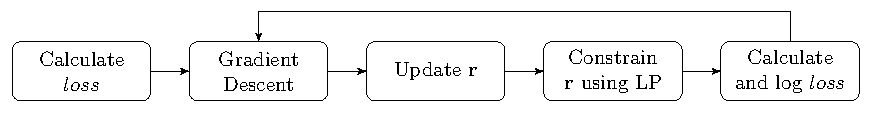
\includegraphics[width=\textwidth]{logic_alg_pricing}
        \caption{Logic Flow of Algorithm \ref{alg:Solving the Pricing Problem}}
        \label{fig:Logic Flow of Algorithm Pricing Problem}
    \end{figure}
    \begin{algorithm}
        \caption{Solving the Pricing Problem} \label{alg:Solving the Pricing Problem}
        \begin{algorithmic}[1]
            \Function{Forward}{$\matr{D}, \matr{f}, \vect{r}, \matr{w_1}, \matr{w_2}, \vect{x}$}
                \State $\matr{F} \gets \Call{Build-Dataset}{\matr{D}, \matr{f}, \vect{r}}$\Comment{Defined in Algorithm \ref{alg:Constructing the Input Dataset}}
                \State $\matr{O}_1 \gets \text{reLU}(\Call{Batch-Multiply}{\matr{F}, \matr{w_1}})$
                \State $\matr{O}_2 \gets \text{softmax}(\Call{Batch-Multiply}{\matr{O}_1, \matr{w_2}})$
                \State $\matr{P} \gets \matr{O}_2^T$
                \State $\vect{y} \gets \matr{P} \cdot \vect{x}$
                \State \Return $\lVert \vect{y} - \mean{\vect{y}} \rVert / J$
            \EndFunction
            \vspace*{-.7\baselineskip}\Statex\hspace*{\dimexpr-\algorithmicindent-2pt\relax}\rule{\textwidth}{0.1pt}%
            \Statex\hspace*{-\algorithmicindent}\textbf{Main Script}%
            \vspace*{-.6\baselineskip}\Statex\hspace*{\dimexpr-\algorithmicindent-2pt\relax}\rule{\textwidth}{0.1pt}% horizontal rule
            \State $\vect{r} \gets \Call{Random}{\;(J)\;}$\Comment{$\vect{r}$ has dimensions $J$}
            \State $loss \gets \Call{Forward}{\matr{D}, \matr{f}, \vect{r}, \matr{w_1}, \matr{w_2}, \vect{x}}$
            \For{$e = 1, 2, \dots, \text{Epochs}$}
                
            \State $\Call{Gradient-Descent}{loss, \vect{r}}$
            \State $\vect{r} \gets \Call{Update-Using-Gradients}{\vect{r}}$
            \State $\vect{r} \gets \Call{LP}{\vect{r}, \mathcal{R}}$\Comment{LP($\cdot$) explained in \cref{sec:Constraining Rewards}}
            \State $loss \gets \Call{Forward}{\matr{D}, \matr{f}, \vect{r}, \matr{w_1}, \matr{w_2}, \vect{x}}$
            \State $\Call{Log-Best-Rewards}{loss, \vect{r}}$\Comment{Records $\vect{r}$ with the lowest $loss$ yet}
            \EndFor
        \end{algorithmic}
    \end{algorithm}

    \subsubsection{Constraining Rewards} \label{sec:Constraining Rewards}
    After updating the rewards, the program constrains them using LP($\cdot$) such that $\sum_{i}r_i \leq \mathcal{R}$ and $r_i \geq 0$. To do so, the LP($\cdot$) finds another set of rewards $\vect{r'}$ such that the absolute difference between new and old rewards ($\sum_{i}|r'_i - r_i|$) is minimum. The mathematical formulation is given in Equation \ref{eq:lp_math_constrain_rewards}, which was implemented (see \cref{sec:Implementation}) using SciPy's Optimize Module \cite{SCPOptimizeDocs}. Since the module supports a standard format for doing linear programming, Equation \ref{eq:lp_code_constrain_rewards} (after rearranging constraints and building $\matr{A}, \vect{b}$ and $\vect{c}$) is used, which is mathematically equivalent to Equation \ref{eq:lp_math_constrain_rewards}.
    \begin{multicols}{2}
        \begin{equation} \label{eq:lp_math_constrain_rewards}
            \begin{aligned}\\
                & \underset{\vect{r'}}{\text{minimize}}
                & & \sum_{i}|r'_i - r_i|\\
                & \text{subject to}
                & & \sum_{i}r'_i \leq \mathcal{R}\\
                &&& r_i \geq 0\\ \\
            \end{aligned}
        \end{equation}\break
        \begin{equation} \label{eq:lp_code_constrain_rewards}
            \begin{aligned}
                & \underset{[\vect{r'}, \vect{u}]}{\text{minimize}}
                & & \sum_{i} u_i\\
                & \text{subject to}
                & & r'_i - r_i \leq u_i\\
                &&& r_i - r'_i \leq u_i\\
                &&& \sum_{i} r'_i \leq \mathcal{R}\\
                &&& r'_i, u_i \geq 0
            \end{aligned}
        \end{equation}
    \end{multicols}
    
    \section{Experiment Specifications} \label{sec:Experiment Specifications}
    \begin{mydef} \label{def:GPU Speedup}
        GPU Speedup: Ratio of time elapsed with GPU ``set'' and that with CPU ``set''. Time taken to transfer data from CPU to GPU is included in calculating GPU ``set'' time elapsed. (Speedup = $\frac{CPU-time}{GPU-time\; +\; Transfer-time}$)
    \end{mydef}
    To test both our models, we conducted several tests for optimization and GPU speedup over CPU. After initializing all parameters randomly and reading data from files, the models were run for 1000 to 10000 epochs depending on the complexity of the model and any potential benefits emerging with more epochs.
    
    Hardware specifications and software versions used for the experiments are listed in Table \ref{tab:Hardware Specifications and Software Versions Used for Experiments}. We conducted two types of tests: optimization tests on original datasets and GPU speedup tests on randomly generated datasets. The random dataset of 116 locations ($J$) and 173 time units ($T$) was generated beforehand using NumPy (without any seed). We believe that speedup tests on original datasets would give similar results, though we used randomly generated datasets because it was easier to scale and build random datasets of different batch-sizes for testing. The models were timed for the executed operations in a neural network and the LP, including transfer times of tensors between the RAM and GPU's memory. Time taken for preprocessing was ignored. We also clarify that runtimes given in Results (\cref{sec:Results}) can differ based on other running processes and threads while doing experiments. However, one should obtain similar GPU speedup results when doing the experiments again.
    \begin{table}[!htbp]
        \centering
        \caption{Hardware Specifications and Software Versions Used for Experiments}
        \label{tab:Hardware Specifications and Software Versions Used for Experiments}
        \begin{tabular}{|c|c|}
            \hline
            \multicolumn{2}{c}{\textbf{Hardware}}\\
            \hline
            \textbf{Type} & \textbf{Unit/Specs}\\
            \hline
            Desktop & Dell Precision Tower 3620\\
            CPU & Intel Core i7-7700K\\
            RAM & 16GB\\
            GPU & NVIDIA Quadro P4000\\
            \hline
        \end{tabular}\quad
        \begin{tabular}{|c|c|}
            \hline
            \multicolumn{2}{c}{\textbf{Software}}\\
            \hline
            \textbf{Library/Package} & \textbf{Version}\\
            \hline
            Ubuntu OS & 16.04.2 LTS\\
            CUDA & 8.0\\
            cuDNN & 5.1.10\\
            MKL & 2017.0.3\\
            Python & 2.7.13 (Anaconda)\\
            PyTorch & 0.1.12\textunderscore2\\
            NumPy & 1.12.1\\
            SciPy & 0.19.0\\
            \hline
        \end{tabular}
    \end{table}
    
    Note that by GPU ``set'' we mean \textit{distributing} operations in the scripts between CPU and GPU, while by CPU ``set'' we mean that the operations were executed \textit{only} on the CPU. Since GPUs are inferior than CPUs at handling most operations other than simple arithmetic matrix ones (see \cref{sec:Computation Using GPUs}), we used - and recommend using - both the CPU and the GPU in the former case (GPU ``set'') to handle operations each is superior at. However, since the models in \cref{sec:Identification Problem} and \cref{sec:Pricing Problem} (not the full scripts) are primarily arithmetic operations on matrices and tensors, it is clear that they were executed on the GPU when it was ``set'' and on the CPU when the CPU was ``set''. Other than this optimization, we did not specifically design any parallelized algorithm for either configurations, relying on the PyTorch Library's and NumPy-SciPy's inbuilt implementation.
    
    On the algorithm side, we used Adam's algorithm for \textsc{Gradient-Descent}($\cdot$), after testing performances of several algorithms including but not limited to Stochastic Gradient Descent (SGD) \cite{SGD}, Adam's Algorithm \cite{Adam} and Adagrad \cite{Adagrad} (PyTorch lets you choose the corresponding function). Since Adam's algorithm was found to work best with both models over all test runs, all experiments were done using Adam's algorithm. Hence, all results were also obtained using Adam's algorithm.
    
    \subsection{Running the Identification Problem's Model} \label{sec:Running the Identification Problem's Model}
    \subsubsection{Optimizing the Original Dataset} \label{sec:Identification Problem-Optimizing the Original Dataset}
    The 3-layered neural network was run for 10000 epochs on the original dataset, which was split 80:20 for training and testing sets, with different learning rates = $\{10^{-2}, 10^{-3}, 10^{-4}, 10^{-5}\}$. Since we were aiming for optimization, we ran multiple tests (5 different seeds with each learning rate) of the model only with the GPU ``set''.
    
    To compare this model's optimization results with other model structures, the previously studied 2-layered network \cite{Xue2016Avi2} and a 4-layered neural network were used. The 4-layered network had another hidden layer with reLU, equivalent to the hidden layer in the current 3-layered network in Figure \ref{fig:3-dimensional view of the network slice, taking in Fv}. The results from the 2-layered network were obtained from the previous study, and those from the 4-layered network were attained on the same original dataset with same parameter values (learning rates, epochs etc.).
    
    \subsubsection{Testing GPU Speedup on the Random Dataset} \label{sec:Identification Problem-Testing GPU Speedup on the Random Dataset}
    After generating a random dataset, we ran our 3-layered model on with different batch-sizes $T = 17, 51, 85, 129, 173$ ($J = 116$) and different seeds with both GPU and CPU ``set'', logging the elapsed time for model execution. The total time elapsed was averaged for a batch-size on a device, which were used to generate scatter/line plots (see \cref{sec:IdProbRes - GPU}).
    
    \subsection{Running the Pricing Problem's Model} \label{sec:Running the Pricing Problem's Model}
    \subsubsection{Optimizing the Original Dataset} \label{sec:Pricing Problem-Optimizing the Original Dataset}
    After obtaining the set of weights $\matr{w_1}$ and $\matr{w_2}$ optimized using different seeds, we tested to find the best rewards (with the lowest loss - Equation \ref{eq:pricing_problem}) with random $\vect{r}$ initiation. To obtain the best rewards, the model was run on all sets of weights obtained from the Identification Problem for 1000 epochs with different learning rates. In search for the best rewards with the minimum loss, we took this approach:
    \begin{enumerate}
        \item Run differently seeded rewards on all sets of weights (obtained from the Identification Problem) and identify a set of weights which performed better than the others (low $Z_I$ - Equation \ref{eq:pricing_problem}) on average. The learning rate was fixed to $10^{-3}$ in this case.
        \item Use that set of weights to run a number of tests with varying seeds and learning rates = $\{10^{-2}, 5 \times 10^{-3}, 10^{-3}, 5 \times 10^{-4}, 10^{-4}, 5 \times 10^{-5}, 10^{-5}\}$, and choose the resulting rewards which gave the lowest loss value $Z_I$.
    \end{enumerate}
    Two sets of rewards were tested for loss values as baseline comparisons to our model - a randomly generated set, and another with elements proportional to the reciprocal of number of visits at each location. While the former was a random baseline, the latter captured the idea of allocating higher rewards to relatively under-sampled locations. The average loss values (on different sets of weights) were compared for all tests with the baselines.
    
    \subsubsection{Testing GPU Speedup on the Random Dataset} \label{sec:Pricing Problem-Testing GPU Speedup on the Random Dataset}
    Using the same random dataset as used before (data doesn't matter as long as it is random), we ran the Pricing Problem's model with different batch-sizes $J = 11, 35, 55, 85, 116$ ($T = 173$) and different seeds with both GPU and CPU ``set''.
    
    Since PyTorch does not provide a GPU-accelerated Simplex LP solver, we relied on SciPy's Optimize Module to solve our LP sub-problem (see \cref{sec:Constraining Rewards}). Since SciPy's implementation does not utilize the GPU, we expected the LP problem to be executed on the CPU and thus deliver equal runtimes in both GPU and CPU ``set'' configurations.
    
    \section{Results} \label{sec:Results}
    \subsection{Identification Problem's Results} \label{sec:Identification Problem's Results}
    \subsubsection{Optimization Results} \label{sec:IdProbRes - Optimization}
    Running the 3-layered network with the GPU ``set'' with different learning rates on different seeds (to calculate average performance of each learning rate) for 10000 epochs showed that the model performing the best with learning rate = $10^{-3}$. 
    
    We observed that higher learning rates ($>10^{-2}$) could only decrease the loss function ($Z_I$ - Equation \ref{eq:iden_problem}) to a limit, after each the updates in the weights caused the loss function to oscillate and increase. This phenomena is exemplified in Figure \ref{fig:Test Loss Plots of Different Learning Rates to Find Weights}, which are plots of different models with the same seed but different learning rates. On the other side of $10^{-3}$, lower learning rates took too long to train. Runtime for the model on 10000 epochs was an average 1232.56 seconds (20 runs = 5 seeds $\times$ 4 learning rates), and models with learning rates $< 10^{-3}$ did not perform better than those with learning rate = $10^{-3}$ on \textit{any} run. Although the decrease in test losses were constant for learning rates $< 10^{-3}$, we feel that they may be computationally expensive and temporally inconvenient to train.
    \begin{table}[!htbp]
        \centering
        \caption[Loss Values Calculated for Different Models for Identification Problem]{Loss Values Calculated for Different Models for Identification Problem: For both the 3- and the 4-layered models, learning rate = $10^{-3}$ outperformed other learning rates. Consequently, that learning rate is used in comparison with other models in Figure \ref{fig:Comparison of Loss Values from Different Models of the Identification Problem}.}
        \label{tab:Loss Values Calculated for Different Models for Identification Problem}
        \begin{tabular}{c | c | c}
            \hline
            \multirow{2}{*}{\textbf{Learning Rate}} & \multicolumn{2}{c}{\textbf{Average Test Loss Values}} \\
            & 3-layered & 4-layered\\
            \hline
            $10^{-2}$ & 0.168 $\pm$ 0.068 & 0.494 $\pm$ 0.083\\
            $10^{-3}$ & \textbf{0.119 $\pm$ 0.016} & \textbf{0.228 $\pm$ 0.048}\\
            $10^{-4}$ & 0.151 $\pm$ 0.040 & 0.237 $\pm$ 0.067\\
            $10^{-5}$ & 0.212 $\pm$ 0.040 & 0.320 $\pm$ 0.067\\
            \hline
        \end{tabular}
    \end{table}
    
    Table \ref{tab:Loss Values Calculated for Different Models for Identification Problem} gives the average \textit{end} test loss results. Observing that the average test loss values of learning rate = $10^{-3}$ is the lowest, we compare its results with the previous study's 2-layered network, historical data \cite[// todo]{Xue2016Avi2}, and a 4-layered network with learning rate = $10^{-3}$ (see \cref{sec:Identification Problem-Optimizing the Original Dataset}).
    
    \begin{figure}[!htbp]
        \centering
        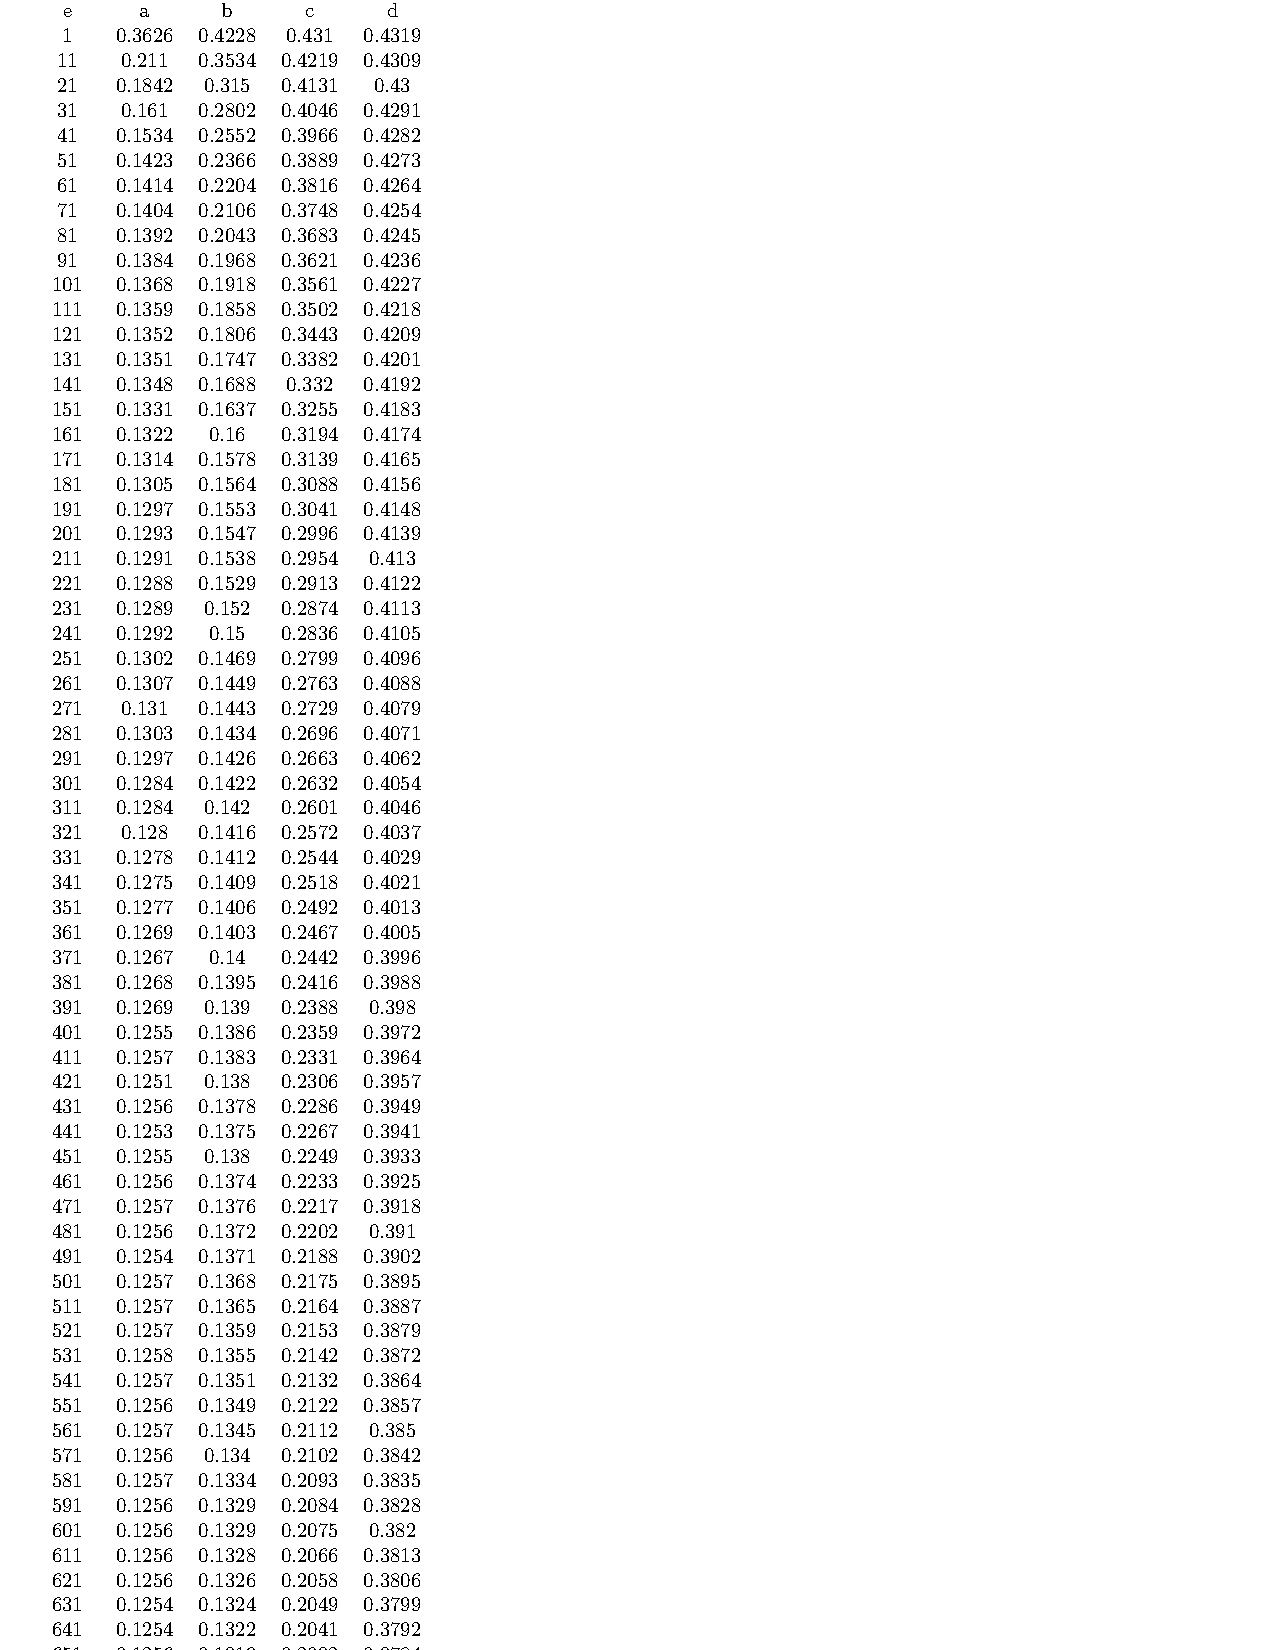
\includegraphics[width=16cm, height=10cm]{test_losses_diff_lr_plot}
        \caption{Test Loss Plots of Different Learning Rates to Find Weights}
        \label{fig:Test Loss Plots of Different Learning Rates to Find Weights}
    \end{figure}
    \begin{figure}[!htbp]
        \centering
        \begin{minipage}{.49\textwidth}
            \centering
            \begin{tikzpicture}
                \begin{axis}[
                    ybar,
                    width=\textwidth,
                    enlarge x limits=0.15,
                    legend style={at={(0.02,0.98)},
                        anchor=north west,legend columns=1},
                    ylabel={Loss Value},
                    symbolic x coords={2-layer,3-layer,4-layer, Historical},
                    xtick=data,
                    nodes near coords,
                    nodes near coords align={vertical},
                    every node near coord/.style={/pgf/number format/fixed},
                    xlabel={Models},
                    xlabel style={yshift=-.5cm}
                ]
                \addplot coordinates {(2-layer,0.26) (3-layer,0.12) (4-layer,0.23) (Historical, 0.36)};% test set
                \addplot coordinates {(3-layer,0.03) (4-layer,0.06)};% training set
                \legend{Test Set,Training Set}
                \end{axis}
            \end{tikzpicture}
            \caption[Comparison of Loss Values from Different Models of the Identification Problem]{Comparison of Loss Values from Different Models of the Identification Problem: Loss values for the training set are inevitably lower than that for the test set, which should be the basis for comparison}
            \label{fig:Comparison of Loss Values from Different Models of the Identification Problem}
        \end{minipage}\hfill
        \begin{minipage}{.49\textwidth}
            \centering
            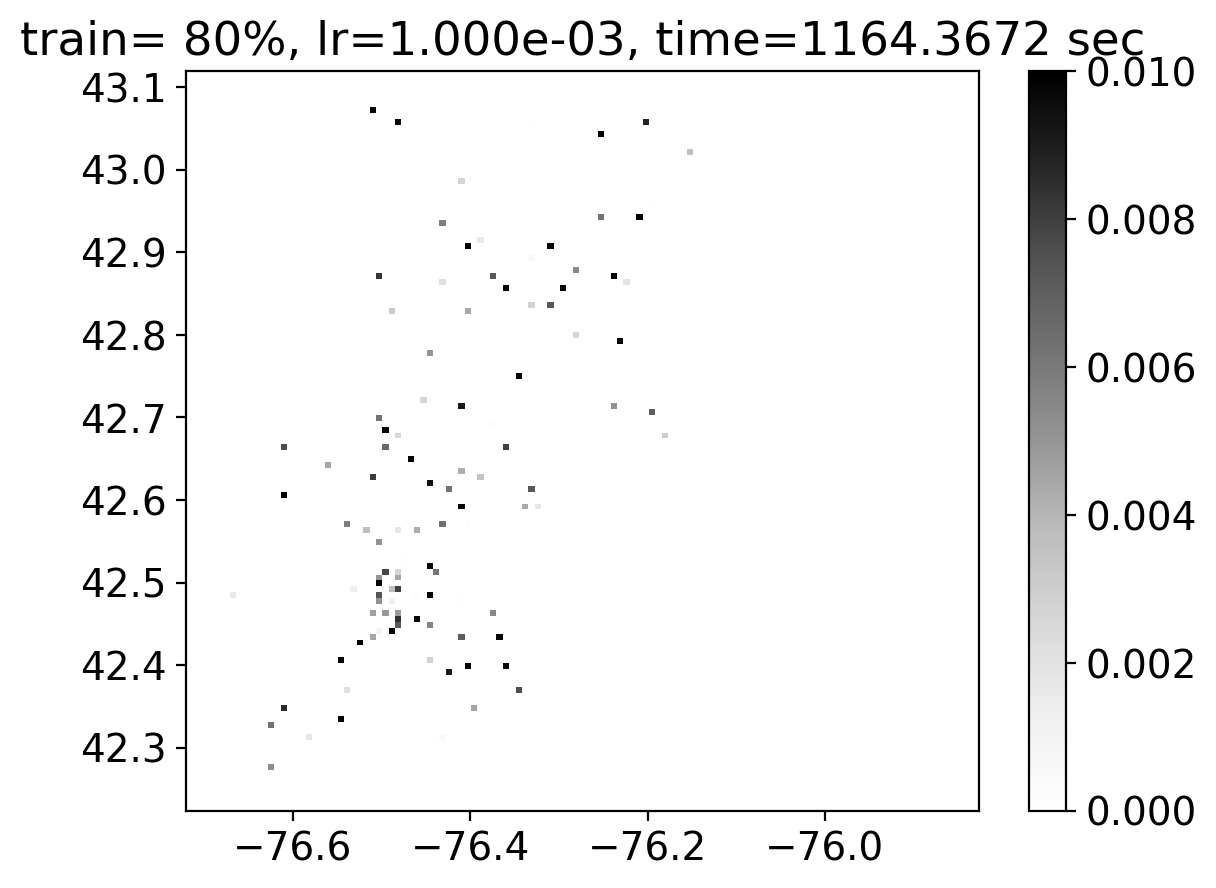
\includegraphics[width=\textwidth]{weights_map_plot_3}
            \caption[Predicted Probabilities of Agents Visiting Each Location Plotted on a Map (Latitude, Longitude) Representing Tompkins and Cortland Counties, NY]{Predicted Probabilities of Agents Visiting Each Location Plotted on a Map (Latitude, Longitude) Representing Tompkins and Cortland Counties, NY: Dark dots represent high prediction of visits. This can be compared to the plots for the 2-layered network and other models \cite[Figure 3]{Xue2016Avi2}.}
            \label{fig:Predicted Probabilities of Agents Visiting Each Location Plotted on a Map}
        \end{minipage}
    \end{figure}

    As depicted in Figure \ref{fig:Comparison of Loss Values from Different Models of the Identification Problem}, our 3-layered neural network outperformed the previous 2-layered model by \textbf{0.14 units (14\% more closer to Ground Truth - $\matr{y}$)} \cite[Table 1]{Xue2016Avi2}, and also produced much better results (12\% more closer to Ground Truth) than the 4-layered model.
    
    We also generated the predicted probabilities of the agents visiting each location ($\matr{P} \cdot \matr{x}$) in the Test Set, and plotted it onto a map marked by the locations' latitudes and longitudes. Figure \ref{fig:Predicted Probabilities of Agents Visiting Each Location Plotted on a Map} shows such a plot generated by the 3-layered network, where each dot represents a location.
    
    Although there remained a $\approx$ 9\% difference (0.09 loss units) in the values of training and testing set, the 3-layered model was not starkly overfitting as an average \textit{end} difference of $8.76\pm1.59\%$ persisted for many epochs, instead of increasing and tuning more to the training set. This case was similar for the 4-layered model, producing an average \textit{end} difference of $16.77 \pm 4.73\%$. This result is shown in Figure \ref{fig:Train & Test Loss Values' Plots of Different Models} with plots of loss values at each epoch for the 3- and the 4-layered network. On a side note, learning rates greater than $10^{-3}$ led to high oscillation and some overfitting in both models.
    \begin{figure}[!htbp]
        \centering
        \begin{subfigure}{.49\textwidth}
            \centering
            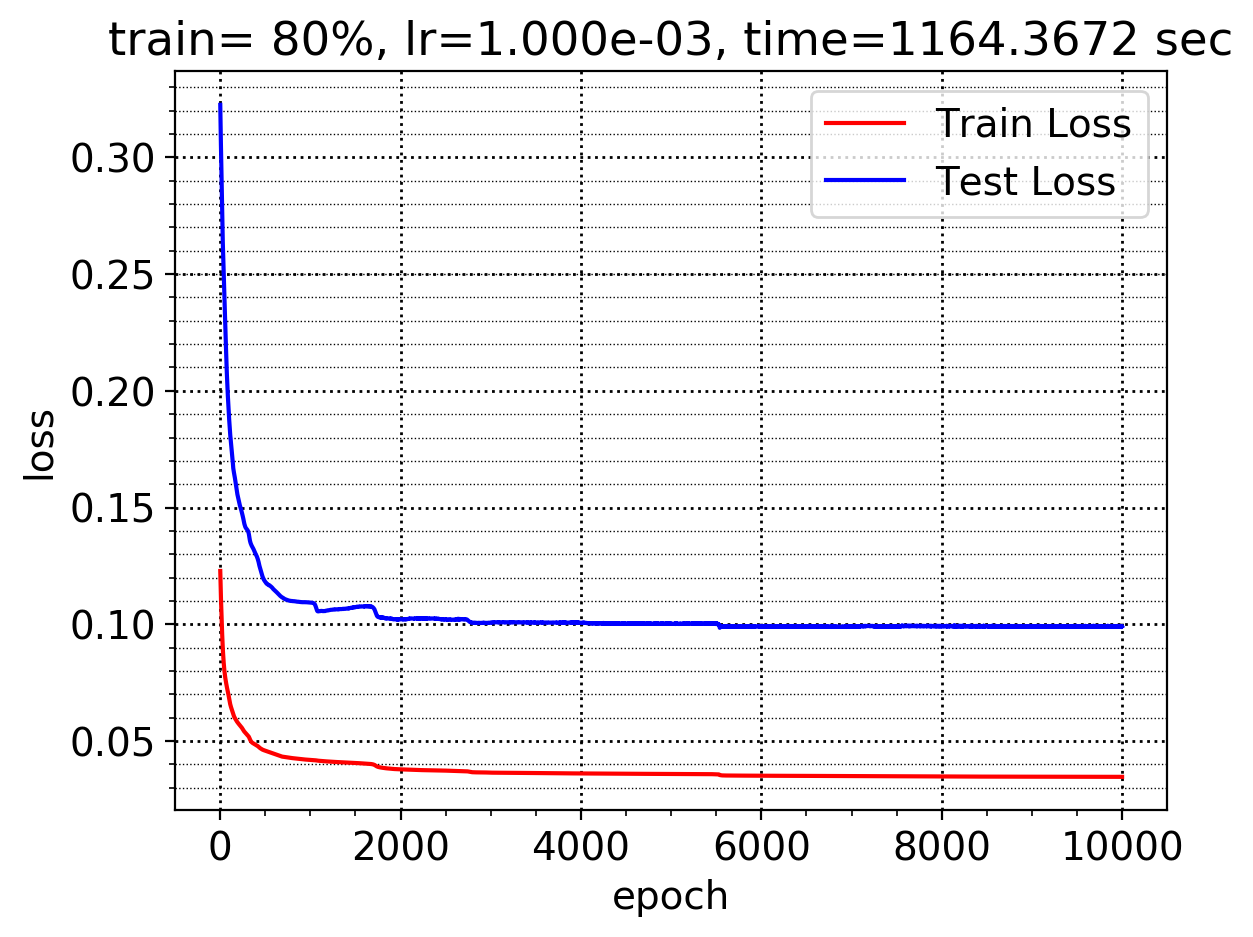
\includegraphics[width=\textwidth]{weights_train_test_loss_3_plot}
            \caption{Plot for 3-layered Model}
            \label{fig:Plot for 3-layered Model}
        \end{subfigure}
        \begin{subfigure}{.49\textwidth}
            \centering
            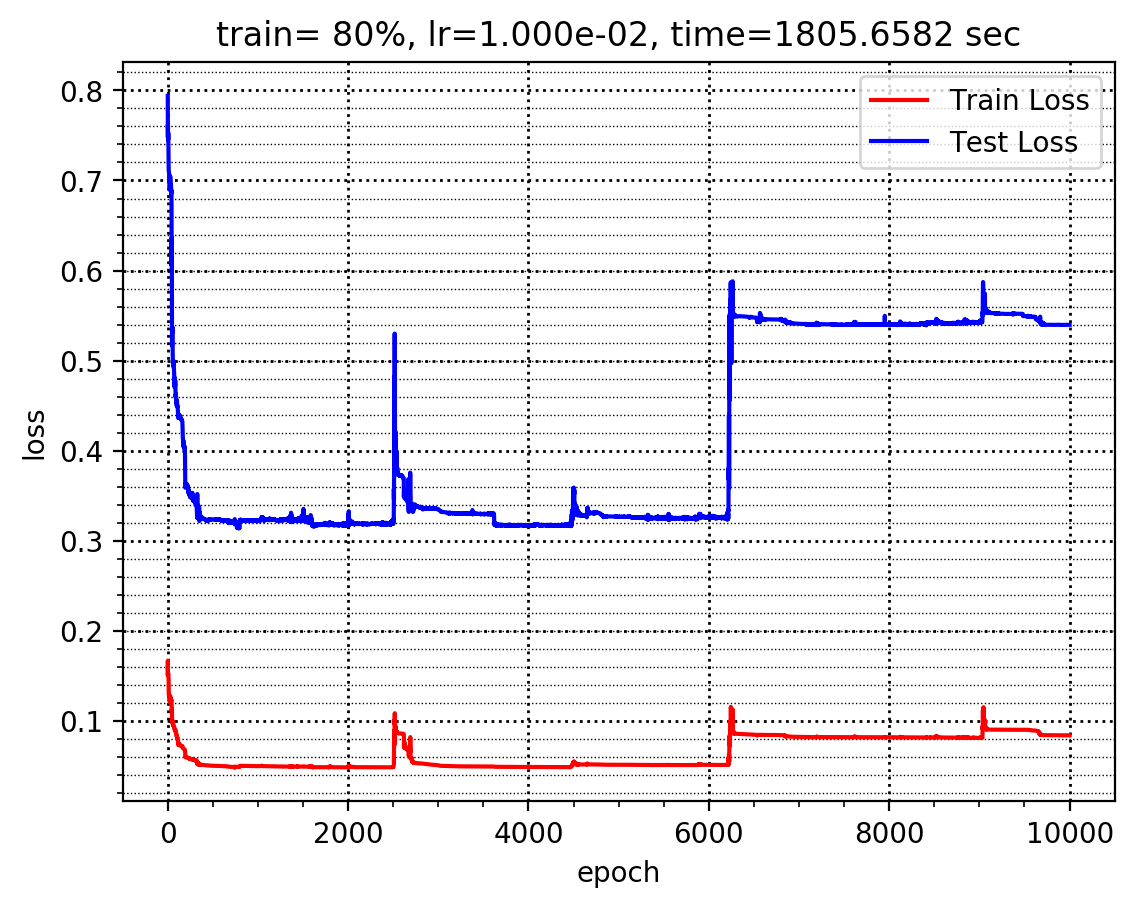
\includegraphics[width=\textwidth]{weights_train_test_loss_4_plot}
            \caption{Plot for 4-layered Model // todo}
            \label{fig:Plot for 4-layered Model}
        \end{subfigure}
        \caption[Train \& Test Loss Values' Plots for One of the Runs of Different Models]{Train \& Test Loss Values' Plots for One of the Runs of Different Models: Both networks learn the set of weights quickly, as displayed in the steep descent in loss values before $\approx$ 1000 epochs. This quick learning is due to the choice of \textsc{Gradient-Descent}($\cdot$) function - Adam's algorithm \cite{Adam}. Other algorithms like SGD \cite{SGD} and Adagrad \cite{Adagrad} learn relatively slowly.}
        \label{fig:Train & Test Loss Values' Plots of Different Models}
    \end{figure}

    \subsubsection{GPU Speedup Results} \label{sec:IdProbRes - GPU}
    Running on batches of sizes $T = 17, 51, 85, 129, 173$ on a randomly generated dataset for 1000 epochs, with both GPU and CPU ``set'' separately, we obtained information on full execution runtimes (including both training and testing). The average results (over 3 different seeds for each batch) are plotted in Figure \ref{fig:Execution Times of Different Batch-Sizes with GPU and CPU ``set'' Separately}, which show promising GPU speedup over CPU figures for any batch size; the GPU speedup averaged over all tested batch-sizes is \textbf{9.06$\pm$0.45}.
    \begin{figure}[!htbp]
        \centering
        \begin{subfigure}{.59\textwidth}
            \begin{tikzpicture}
            \begin{axis}[
            width=\textwidth,
            height=8cm,
            xtick=data,
            xlabel={Batch-Size $T$},
            ylabel={Time/s},
            enlarge x limits=0.15,
            y tick label style={/pgf/number format/1000 sep=},
            extra y tick style={grid=major, tick label style={xshift=-1cm}},
            legend style={at={(0.02,.98)},
                anchor=north west},
            nodes near coords,
            ]
            \addplot+ [mark=*,error bars/.cd, y dir=both,y explicit] coordinates {
                (17,118.23) +- (1.77, 1.77)
                (51,345.33) +- (2.00, 2.00)
                (85,547.59) +- (1.76, 1.76)
                (129,871.01) +- (3.01, 3.01)
                (173,1095.24) +- (1.71, 1.71)
            };  % cpu
            \addplot+ [mark=*,error bars/.cd, y dir=both,y explicit] coordinates {
                (17,12.56) +- (0.022, 0.022)
                (51,35.85) +- (0.232, 0.232)
                (85,59.12) +- (0.131, 0.131)
                (129,107.95) +- (12.788, 12.788)
                (173,122.72) +- (0.169, 0.169)
            };  % gpu
            \legend{CPU ``set'',GPU ``set''}
            \end{axis}
            \end{tikzpicture}
        \end{subfigure}
        \begin{subfigure}{.4\textwidth}
            \centering
            \begin{tikzpicture}
                \begin{axis}[
                ybar,
                width=\textwidth,
                height=8cm,
                xtick=data,
                xlabel={Batch-Size $T$},
                ylabel={GPU Speedup},
                ymin=0,
                enlarge x limits=0.15,
                extra y tick style={grid=major, tick label style={xshift=-1cm}},
                nodes near coords,
                ]
                \addplot+ coordinates {
                    (17,9.41)
                    (51,9.63)
                    (85,9.26)
                    (129,8.07)
                    (173,8.92)
                };
                \legend{}
                \end{axis}
            \end{tikzpicture}
        \end{subfigure}
        \caption[Finding Weights - Execution Times of Different Batch-Sizes $T$ with GPU and CPU ``set'' Separately]{Finding Weights - Execution Times of Different Batch-Sizes $T$ with GPU and CPU ``set'' Separately: The GPU delivers faster computation than CPU even as the datasets' sizes grow - the average speedup is 9.06$\pm$0.45. Also, the error bars are indiscernible because they are too small ($< 1\%$)}.
        \label{fig:Execution Times of Different Batch-Sizes with GPU and CPU ``set'' Separately}
    \end{figure}

    \subsection{Pricing Problem's Results} \label{sec:Pricing Problem's Results}
    \subsubsection{Optimization Results} \label{sec:PriProbRes - Optimization}
    Taking the approach mentioned in \cref{sec:Pricing Problem-Optimizing the Original Dataset}, different sets of weights gave consistent loss values (even with differently seeded rewards). The best was the set-2 of weights, using which the average loss value for the Pricing Problem hovered around 0.0079\%. Next, running differently seeded rewards with different learning rates on set-2 of weights, which performed the best, we obtained the \textbf{lowest loss value of 0.0068\%}.
%    \begin{figure}[!htbp]
%        \centering
%        \begin{tikzpicture}
%        \begin{axis}[
%        ybar,
%        width=.6\textwidth,
%        height=7cm,
%        enlarge x limits=0.15,
%        ylabel={Loss Value (in \%)},
%        symbolic x coords={Set-1,Set-2,Set-3,Set-4,Set-5},
%        xtick=data,
%        nodes near coords,
%        nodes near coords align={vertical},
%        xlabel={Models},
%        xlabel style={yshift=-.5cm}
%        ]
%        \addplot+ [error bars/.cd, y dir=both, y explicit] coordinates {
%            (Set-1, 0.0152) +- (0.0001, 0.0001)
%            (Set-2, 0.0079) +- (0.0005, 0.0005)
%            (Set-3, 0.0139) +- (0.0003, 0.0003)
%            (Set-4, 0.0129) +- (0.0002, 0.0002)
%            (Set-5, 0.0155) +- (0.0002, 0.0002)
%        };
%        \end{axis}
%        \end{tikzpicture}
%    \end{figure}

    Compared to the proportional reward distribution (loss values calculated using set-2 of weights), our model optimized the rewards such that the loss value was $\approx$ \textbf{3 times} lower. We should also clarify that we compare the best loss values, as the organizer expects to find a distribution that is as optimal as possible. Table \ref{tab:Loss Values Calculated from Different Sets of Rewards} lists the best loss values obtained on each type of reward allocation (model's predicted, random and proportional - \cref{sec:Pricing Problem-Optimizing the Original Dataset}).
    \begin{table}[!htbp]
        \centering
        \caption[Loss Values Calculated from Different Sets of Rewards]{Loss Values Calculated from Different Sets of Rewards: The values are small because the loss function $Z_P(\vect{r})$ (Equation \ref{eq:pricing_problem}) is averaged over the number of locations}
        \label{tab:Loss Values Calculated from Different Sets of Rewards}
        \begin{tabular}{|c|c|}
            \hline
            \textbf{Rewards Obtained From} & \textbf{Best Loss Values (In \%)}\\
            \hline
            Model's Prediction & 0.0068\\
            Random Initialization & 0.0331\\
            Proportional Distribution & 0.0235\\
            \hline
        \end{tabular}
    \end{table}
    
    \subsubsection{GPU Speedup Results} \label{sec:PriProbRes - GPU}
    After running on different batch-sizes $J = 11, 35, 55, 85, 116$, we \textbf{did not observe radical speedup} for the full model. Figure \ref{fig:Finding Rewards - Time Taken by the Full Model} shows the decreasing speedup trend, as the GPU ``set'' configuration started struggling to complete all epochs faster than with CPU ``set''. GPU Speedup for the full model was a mere \textbf{1.53 $\pm$ 0.10}, with the GPU ``set'' config. giving better results as the dataset increased. 
    
    Since the the low GPU speedup was uncanny, we looked for operations that were causing the program to slow down on the GPU. Guessing that the LP problem (Equations \ref{eq:lp_math_constrain_rewards} \& \ref{eq:lp_code_constrain_rewards}) might be influencing the runtimes, we recorded execution times for both the neural network and the LP separately. As we suspected, the LP \textit{did} impact the runtime more than the neural networks did, while the GPU speedup for the Neural Network was expectedly high with \textit{only} with large batch-sizes (Figure \ref{fig:Finding Rewards - Time taken by the Neural Network}). The time elapsed for the Neural Network includes time taken to transfer tensors to and from the GPU, which results in overhead - as seen in higher runtime for lower batch-sizes in Figure \ref{fig:Finding Rewards - Time taken by the Neural Network}. However, as the batch-sizes grew, we see the computation dominating over the transfer time, resulting in higher CPU ``set'' runtimes; the GPU ``set'' runtimes almost grow linearly for the tested batch-sizes.
    \begin{figure}[!htbp]
        \centering
        \begin{subfigure}{\textwidth}
            \centering
            \begin{tikzpicture}
                \begin{axis}[
                    width=12cm,
                    height=8cm,
                    xtick=data,
                    xlabel={Batch-Size $J$},
                    ylabel={Time/s},
                    enlargelimits=0.15,
                    y tick label style={/pgf/number format/1000 sep=},
                    extra y tick style={grid=major, tick label style={xshift=-1cm}},
                    legend style={at={(0.02,.98)},
                        anchor=north west},
                    nodes near coords,
                    every node near coord/.append style={yshift=-0.7cm}
                ]
                \addplot+ [mark=*,
                nodes near coords=\raisebox{0.8cm}{\pgfmathprintnumber\pgfplotspointmeta},error bars/.cd, y dir=both,y explicit
                ] coordinates {
                    (11,13.08) +- (1.04, 1.04)
                    (35,50.51) +- (1.73, 1.73)
                    (55,88.95) +- (0.35, 0.35)
                    (85,185.34) +- (0.95, 0.95)
                    (116,346.34) +- (1.67, 1.67)
                };  % cpu
                \addplot+ [mark=*,error bars/.cd, y dir=both,y explicit] coordinates {
                    (11,9.72) +- (0.08, 0.08)
                    (35,33.97) +- (0.26, 0.26)
                    (55,58.97) +- (0.19, 0.19)
                    (85,119.50) +- (0.35, 0.35)
                    (116,197.80) +- (4.02, 4.02)
                };  % gpu
                \legend{CPU ``set'',GPU ``set''}
                \end{axis}
            \end{tikzpicture}
            \caption{Time Taken by the Full Model: GPU Speedup over \textit{all} batch-sizes is only \textbf{1.53 $\pm$ 0.10}.}
            \label{fig:Finding Rewards - Time Taken by the Full Model}
        \end{subfigure}\vspace*{1em}
        \begin{subfigure}{.49\textwidth}
            \centering
            \begin{tikzpicture}
                \begin{axis}[
                    width=\textwidth,
                    height=8cm,
                    xtick=data,
                    enlargelimits=0.15,
                    xlabel={Batch-Size $J$},
                    ylabel={Time/s},
                    y tick label style={/pgf/number format/1000 sep=},
                    extra y tick style={grid=major, tick label style={xshift=-1cm}},
                    legend style={at={(0.02,.98)},
                        anchor=north west},
                    nodes near coords,
                    every node near coord/.append style={yshift=-0.7cm}
                ]
                \addplot+ [mark=*,
                nodes near coords=\raisebox{0.8cm}{\pgfmathprintnumber\pgfplotspointmeta},error bars/.cd, y dir=both,y explicit
                ] coordinates {
                    (11,11.93) +- (0.94, 0.94)
                    (35,48.76) +- (1.68, 1.68)
                    (55,86.49) +- (0.36, 0.36)
                    (85,180.60) +- (0.97, 0.97)
                    (116,336.23) +- (1.46, 1.46)
                };  % cpu
                \addplot+ [mark=*,error bars/.cd, y dir=both,y explicit] coordinates {
                    (11,7.14) +- (0.08, 0.08)
                    (35,31.06) +- (0.26, 0.26)
                    (55,55.81) +- (0.19, 0.19)
                    (85,115.80) +- (0.35, 0.35)
                    (116,193.66) +- (4.02, 4.02)
                };  % gpu
                \legend{CPU ``set'',GPU ``set''}
                \end{axis}
            \end{tikzpicture}
            \caption[Time taken by the LP]{Time taken by the LP: GPU Speedup over \textit{all} batch-sizes is only \textbf{1.62 $\pm$ 0.07}. As discussed in \cref{sec:PriProbRes - GPU} and \cref{sec:Strange GPU Speedup in LP Computation}, we shouldn't have witnessed this speedup as both configurations' LPs were computed on the CPU. Hence, we expected the speedup value to be $\approx$ 1. }
            \label{fig:Finding Rewards - Time taken by the LP}
        \end{subfigure}\hspace*{1em}
        \begin{subfigure}{.49\textwidth}
            \centering
            \begin{tikzpicture}
                \begin{axis}[
                    width=\textwidth,
                    height=8cm,
                    xtick=data,
                    xlabel={Batch-Size $J$},
                    ylabel={Time/s},
                    y tick label style={/pgf/number format/1000 sep=},
                    extra y tick style={grid=major, tick label style={xshift=-1cm}},
                    legend style={at={(0.02,.98)},
                        anchor=north west},
                    nodes near coords,
                    every node near coord/.append style={yshift=-0.65cm}
                ]
                \addplot+ [mark=*,error bars/.cd, y dir=both,y explicit] coordinates {
                    (11,1.15) +- (0.10, 0.10)
                    (35,1.75) +- (0.05, 0.05)
                    (55,2.46) +- (0.01, 0.01)
                    (85,4.74) +- (0.03, 0.03)
                    (116,10.11) +- (0.26, 0.26)
                };  % cpu
                \addplot+ [mark=*,
                nodes near coords=\raisebox{1.2cm}{\pgfmathprintnumber\pgfplotspointmeta}, error bars/.cd, y dir=both,y explicit] coordinates {
                    (11,2.57) +- (0.01, 0.01)
                    (35,2.91) +- (0.01, 0.01)
                    (55,3.16) +- (0.01, 0.01)
                    (85,3.70) +- (0.004, 0.004)
                    (116,4.13) +- (0.001, 0.001)
                };  % gpu
                \legend{CPU ``set'',GPU ``set''}
                \end{axis}
            \end{tikzpicture}
            \caption{Time taken by the Neural Network: GPU Speedup over \textit{all} batch-sizes is only \textbf{1.11 $\pm$ 0.60} - mostly due to high transfer times even for low batch-sizes. However, as batch-sizes grow, computation time dominates over transfer time - GPU ``set'' performs better than CPU ``set''.}
            \label{fig:Finding Rewards - Time taken by the Neural Network}
        \end{subfigure}
        \vspace*{1em}
        \caption[Finding Rewards - Execution Times of Different Batch-Sizes $J$ with GPU and CPU ``set'' Separately]{Finding Rewards - Execution Times of Different Batch-Sizes $J$ with GPU and CPU ``set'' Separately: Scaling is strongly hampered by the LP solver. Comparing the contributions of LP and Neural Network to total runtime on GPU ``set'', \textbf{LP accounts for 90.88 $\pm$ 6.95 \% of the total time.}}
        \label{fig:Finding Rewards - Execution Times of Different Batch-Sizes J with GPU and CPU ``set'' Separately}
    \end{figure}

    \paragraph{Strange GPU Speedup in LP Computation}
    Although the Speedup might seem foreseeable, it is exceptional not expected as we intentionally transferred the needed matrices/tensors to the CPU. SciPy's Optimize Module does not utilize the GPU conspicuously, and we expected similar runtimes for both configurations. However, since this result is not directly relevant to our goal (which is to focus on GPU computation), we pursue reasons in \cref{sec:Strange GPU Speedup in LP Computation} instead of digressing here.
    
    \section{Conclusion} \label{sec:Conclusion}
    Our models for the Identification and the Pricing Problem outperformed previously studied ones \cite{Xue2016Avi2} and other baseline comparisons. For the Identification Problem, the average loss value was 14\% lower than the previous 2-layered model, and 12\% better than the 4-layered model, giving us better results than any other tested model. While we did not test deeper networks, we contend that using more hidden layers will only aggravate overfitting and won't provide better results - as is the case with the 4-layered network. The Pricing Problem's model also delivered at least 3x lower loss values than other baseline comparisons for reward distribution. Clearly, our model outperformed other models in both problems.
    
    On the other hand, we can definitively conclude that the Identification Problem ran faster on the GPU than the CPU, mainly because the model was based on tensors. The Pricing Problem's neural network only performed better with higher batch-sizes, with transfer times hampering performance on lower batch-sizes. With an approximate GPU speedup of 9.06 for the Identification Problem, we can scale to large datasets more efficiently on the GPU than the CPU. Although the Pricing Problem's model only delivered a speedup of $\approx$ 1.53 (with the LP problem heavily impacting the runtime), the 2-layered network for finding rewards gave a speedup of 1.11 $\pm$ 0.60. (mean over all tested batch-sizes). This shows that neural network are inherently quick to optimize on a GPU, if the batch-sizes are large enough. One can further use a GPU-accelerated LP solver or model the LP in the network itself (if possible) to get faster results. On the other hand, using newer generation GPUs and CPUs can undoubtedly solve the problems faster.
    
    \subsection{Interesting Inferences}
    One may also notice compelling reflections from the results. Although some models perform better than others, they bring out similar, interesting inferences:
    \begin{itemize}
        \item One interesting observation in Table \ref{tab:Loss Values Calculated from Different Sets of Rewards} is that the Loss Value from the Proportional Distribution (0.161\%) and Random Initialization (0.160\%) are very close, highlighting that the set of weights obtained from the Identification Problem are dependent on other factors ($\matr{f}, \matr{D}$) as well and not just rewards. In other words, incentivizing under-sampled locations more is as good as random distribution of rewards - as agents don't get more heavily influenced by rewards than any other factor to visit locations.\\
        Moreover, by looking at the model's generated rewards, one can infer that the model chooses to place large rewards in 
    \end{itemize}

    \subsection{Further Research}
    There exist numerous possibilities for solving the problems better and faster - from more complex models to better preprocessing. Some important suggestions are listed below:
    
    \paragraph{Choice of Gradient-Descent Algorithm} Figure \ref{fig:Plot for 3-layered Model} shows how the choice of Adam's algorithm \cite{Adam} for \textsc{Gradient-Descent}($\cdot$) helps the model to learn quickly. However, we also witness long periods of saturation after few epochs. This was the case for several other algorithms (SGD \cite{SGD} and Adagrad \cite{Adagrad}), but with different paces of learning. Since the organizers would want to further optimize the set of weights even, research could be done on avoiding the long, unchanging saturation phase. This may involve using other techniques for \textsc{Gradient-Descent}($\cdot$) (Algorithm \ref{alg:Algorithm for the Identification Problem}) and/or altering the loss function $Z_P(\matr{w_1}, \matr{w_2})$ (Equation \ref{eq:iden_problem}).
    
    \paragraph{Modeling LP Differently to Reduce Runtimes} LP is a simple tool for optimizing different problems, with various algorithms for solving LPs - Simplex, Criss-Cross and other Interior Point techniques. While it gives optimal results, it can be computationally expensive if the matrices are large (as depicted in Figure \ref{fig:Finding Rewards - Time taken by the LP}). One can try several approaches to reduce computation time here:
    \begin{itemize}
        \item Implement GPU Support for the LP. Good CUDA backend support did not exist during our study, forcing us to use SciPy's Optimize Module, which only supported NumPy matrices on the CPU.
        \item Constrain Rewards differently (\cref{sec:Constraining Rewards}). We were unsuccessful in implementing a dual version of the LP, interspersed with the neural network. Nonetheless, constraining rewards using a neural network would drastically improve performance as the current LP accounts for $\approx$ 90 \% of the total runtime.
    \end{itemize}

    \bibliographystyle{IEEEtran}
    \bibliography{IEEEabrv,avicaching}
    
    \cleardoublepage
    \begin{appendices}
    \crefalias{section}{appsec}
    \section{Implementation} \label{app:Implementation}
    The code can be found here[]. \\
    Both the Identification and the Pricing Problem were programmed in Python 2.7 using NumPy 1.12.1, SciPy 0.19.1 and Pytorch 0.1.12 modules [web cites] \cite{SCPOptimizeDocs}\cite{NPDocs}. [Results from Python plotted in Matplotlib 2.0.2] With some code optimizations, the input dataset $\matr{F}$ was built using NumPy's \texttt{ndarray} and Pytorch's \texttt{tensor} functions. Since Pytorch offers NumPy-like code base but with dedicated neural network functions and submodules, Pytorch's \texttt{relu} and \texttt{softmax} functions were used along with other matrix operations.\\
    
    \subsection{Specific Implementation Details for the Pricing Problem}
    Among all the code optimizations in both models, some in that for the Pricing Problem are worth discussing, as they drastically differ from Algorithm \ref{alg:Solving the Pricing Problem} or are intricate. Most optimizations relevant to the Identification Problem are trivial and relate directly to those for the Pricing Problem. Therefore, only those in the Pricing Problem model are discussed.
    
    \subsubsection{Building the Dataset $\matr{F}$}
    Notice that we build the dataset $\matr{F}$ and batch-multiply it with $\matr{w_1}$ on each iteration/epoch (lines 2-3 of Algorithm \ref{alg:Solving the Pricing Problem}). Doing these steps are repetitive as most elements of $\matr{F}$, distances $\matr{D}$ and environmental feature vector $\vect{f}$, do not change unlike rewards $\vect{r}$. Moreover since $\matr{w_1}$ is fixed, Algorithm \ref{alg:Solving the Pricing Problem} would repetitively multiply the $\vect{f}$ and $\matr{D}$ components of $\matr{F}$ with $\matr{w_1}$. To avoid these unnecessary computations, we preprocessed most of $\matr{F}$ by batch-multiplying with $\matr{w_1}$ and only multiplied $\vect{r}$ with the corresponding elements of $\matr{w_1}$. Figure \ref{fig:Splitting and Batch Multiplying F and w1} describes the process graphically.\\
    \begin{figure}[!htbp]
        \centering
        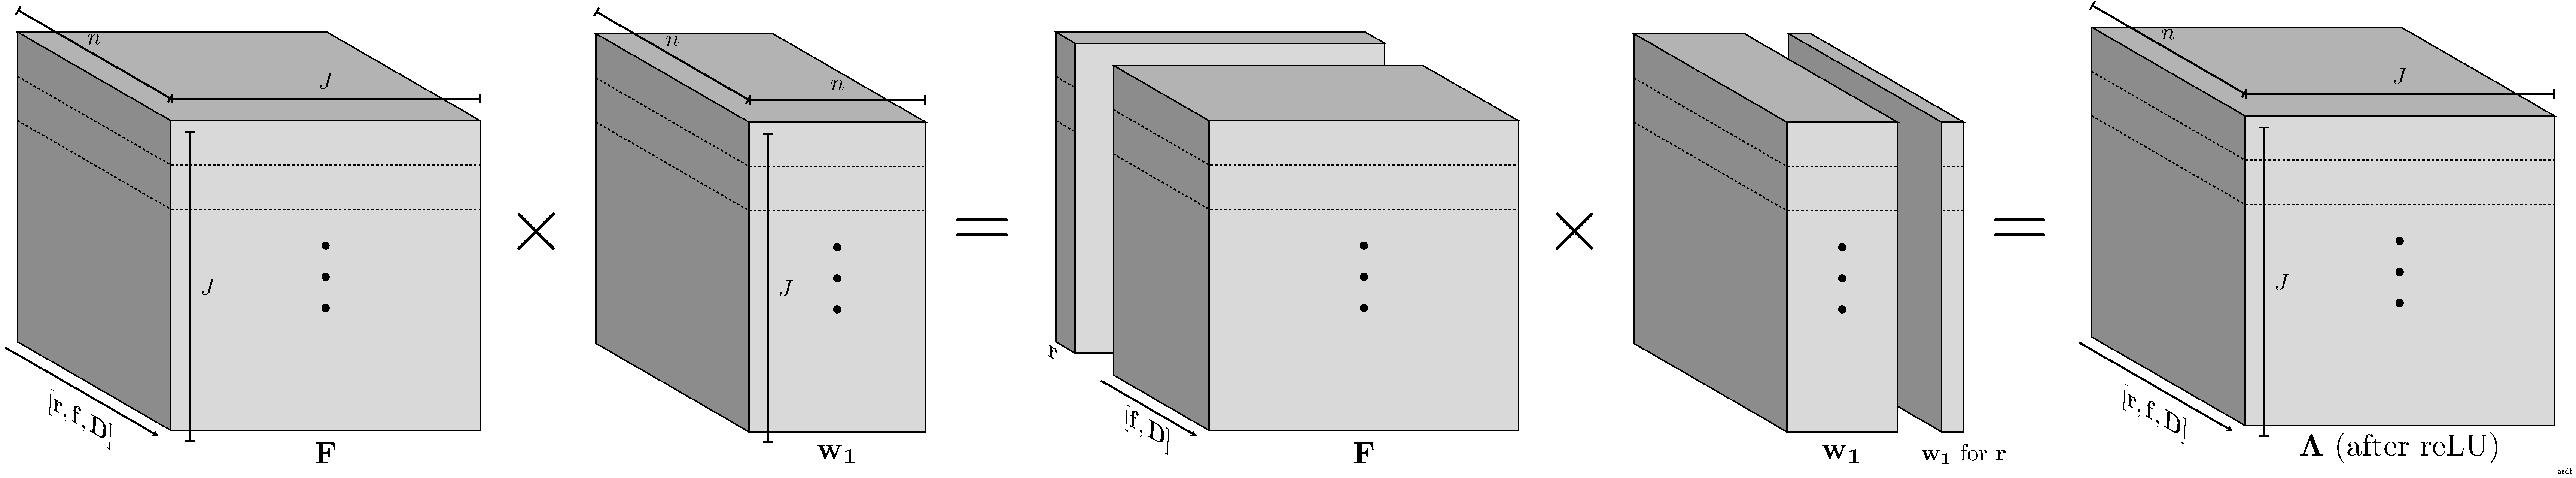
\includegraphics[width=\linewidth]{split_and_batch_multiply}
        \caption{Splitting and Batch Multiplying $\matr{F}$ and $\matr{w_1}$}
        \label{fig:Splitting and Batch Multiplying F and w1}
    \end{figure}    
    Although this preprocessing might seem applicable for the model in Identification Problem too, it does not apply fully. Since the weights $\matr{w_1}$ are updated on each iteration/epoch, we cannot multiply them with parts of $\matr{F}$ beforehand (Algorithm \ref{alg:Algorithm for the Identification Problem}). However, we can combine $\matr{D}$ and $\vect{f}$ in the preprocessing stage and simply append $\vect{r}[t]$ on each iteration, saving computation time.
    
    \subsubsection{Modeling the Linear Programming Problem in the Standard Format}
    The \texttt{scipy.optimize} module's \texttt{linprog} function requires that the arguments are in standard LP format. As discussed in \cref{sec:Calculating Rewards}, Equation \ref{eqn:lp_code_constrain_rewards} resembles the standard format more closely than \ref{eqn:lp_math_constrain_rewards}, but it may not be clear how so.\\
    
    Considering $\vect{u}$ and $\vect{r'}$ as variables $\vect{x}$, Equation \ref{eqn:lp_code_constrain_rewards} translates into Equation \ref{eqn:lp_matrix_rewards} ($J$ is the number of locations).
    \begin{equation} \label{eqn:lp_matrix_rewards}
    \begin{aligned}
    & \text{minimize}
    & & \begin{bmatrix}
    \vect{0_J}\\
    \vect{1_J}\\
    \end{bmatrix}^T
    \begin{bmatrix}
    \vect{r'}\\
    \vect{u}
    \end{bmatrix}\\ \\
    & \text{subject to}
    & & \begin{bmatrix}
    I_J & -I_J\\
    -I_J & -I_J\\
    \vect{1}^T_J & \vect{0}^T_J\\
    \end{bmatrix}
    \begin{bmatrix}
    \vect{r'}\\
    \vect{u}\\
    \end{bmatrix} \leq
    \begin{bmatrix}
    \vect{r}\\
    -\vect{r}\\
    \mathcal{R}\\
    \end{bmatrix}\\
    &&& r'_i, u_i \geq 0
    \end{aligned}
    \end{equation}
    
    \section{Strange GPU Speedup in LP Computation} \label{app:Strange GPU Speedup in LP Computation}
    Even though we intentionally transferred the rewards vector to and constrained it using \texttt{scipy.optimize} module's \texttt{linprog} function on the CPU, we obtained an unexpected GPU Speedup in the LP runtimes (see \cref{sec:PriProbRes - GPU} and Figure \ref{fig:Finding Rewards - Time taken by the LP}). Confounded by this weird behavior, we wanted to pinpoint the reason(s) because SciPy's function could not have differentiated between the configurations and delivered different results. However, since this was not our research's prime motive, we did not take a strong quantitative approach in determining the cause(s).
    
    \subsection{Possible Reasons for GPU Speedup} \label{app:Possible Reasons for GPU Speedup}
    There could have been many reasons for this bizarre behavior, including but not limited to:
    \begin{enumerate}
        \item SciPy's Optimize Module differentiating between configurations. This can be ruled out because the module could not have known the configuration during which it was called. This is because the configuration settings were applicable only on user-programmed operations, and needed to be explicitly stated - as mandated by Pytorch \cite{PTDocs}. SciPy's Optimize Module identifying the configurations is just supernatural.
        \item CPU ``set'' using exploiting more main memory than GPU ``set''. We suspected that since CPU ``set'' configuration's operations were executed solely on the CPU, the residing datasets could have used more main memory than when GPU ``set'' was running. This could have hampered the performance of LP with CPU ``set'', as the LP had lesser space to operate in. Unlike the 1\textsuperscript{st} possibility, this would have meant that CPU ``set'' was slowing down the LP, and not that GPU ``set'' was speeding up the LP.
        \item Neural network in CPU ``set'' using more CPU threads than that in GPU ``set''. The Intel i7-7700K processor is quad-core with 8 threads. Since Pytorch uses OpenMP \cite{PTDocs}, a parallel processing API for CPUs, we fancied the neural network to utilize more threads than that in GPU ``set'', thus allowing less available threads for the LP to run. 
        
        However, given that our scripts in Python did not explicitly use parallel programming with CPU ``set'' and the code was sequential, one could very well suggest that upon completion of the neural network, all threads should have been synchronized, after which the LP would have started. This would have meant that the LP's resources would have been independent of the neural network's resources, raising questions on this possibility.
    \end{enumerate}

    \subsection{LP Slowing Down or Speeding Up?} \label{app:LP Slowing Down or Speeding Up?}
    First we determined whether the LP runtime was being sped up with GPU ``set'' or slowed down with CPU ``set''. To test this, we created a copy of our Pricing Problem's model, which focused only on logging LP runtimes at each epoch. For a baseline comparison, we scripted the same LP \textit{without} the neural network, which gave us the \underline{original} runtimes for the LP (ran for equal number of epochs), without any involvement of Pytorch modules or functions. 
    
    Comparing the former runtimes (CPU and GPU ``set'') with `Only LP' runtime (independent script) in Figure \ref{fig:LP Runtime Example for Different Configurations}, we observed that the LP in the CPU ``set'' configuration took longer to execute than that in  `Only LP' setting during each epoch. We also noticed little to no interaction between the neural network in GPU ``set'' with the LP, as the runtimes of LP in GPU ``set'' were similar to those of LP in `Only LP' setting. This confirmed that CPU ``set'' was slowing down the LP and GPU ``set'' was not speeding it up. But why?
    \begin{figure}[!htbp]
        \centering
        \begin{tikzpicture}
        \begin{axis}[
            width=\textwidth,
            height=8cm,
            xlabel=Epochs,
            ylabel=Time/s,
            scaled y ticks = false,
            grid=both,
            every axis plot/.append style={very thick},
        ]
        \addplot[red] table [col sep=comma,x=epoch, y=cpuset]{datafiles/lp_time_logs.csv};
        \addlegendentry{CPU ``set''}
        
        \addplot[blue] table [col sep=comma,x=epoch, y=gpuset]{datafiles/lp_time_logs.csv};
        \addlegendentry{GPU ``set''}
        
        \addplot[brown] table [col sep=comma,x=epoch, y=onlylp]{datafiles/lp_time_logs.csv};
        \addlegendentry{`Only LP'}
        
        \end{axis}
        \end{tikzpicture}
        \caption[LP Runtime Example for Different Configurations]{LP Runtime Example for Different Configurations: LPs in both CPU and GPU ``set'' start running slowly, but pick up speed after $\approx$ 20 epochs. We could not explain the presence of spikes in LP runtimes of CPU ``set'' and their absence in GPU ``set''. The test was done on a random dataset for 200 epochs, while the other experiment specifications were same as in \cref{sec:Experiment Specifications}.}
        \label{fig:LP Runtime Example for Different Configurations}
    \end{figure}
    
    \subsection{CPU and Main Memory Usage} \label{app:CPU and Main Memory Usage}
    While logging the LP runtimes in \cref{sec:LP Slowing Down or Speeding Up?}, we also recorded an estimate of the amount of computer resources both configurations were using. Using the \texttt{top} package in Ubuntu, we polled the resource monitor every 0.1 seconds while the python script was running\footnote{\label{foo:logs not epochs} Running processes were polled every 0.1 seconds - contributing to a `log'. The longer the script ran, the more logs collected.}. Figures \ref{fig:CPU Usage by Different Configurations} and \ref{fig:Main Memory Usage by Different Configurations} shows how much main memory and CPU resource each setting was using.
    
    It is fascinating to see that CPU ``set'' constantly used more than 4 out of 8 available threads, i.e., $>400\%$ CPU usage, during execution, while GPU ``set'' only used a single thread. Also, since we polled at every 0.1 second, and the LP took a minimum of 0.14 seconds (Figure \ref{fig:LP Runtime Example for Different Configurations}), the data displayed in Figure \ref{fig:CPU Usage by Different Configurations} must show resource use \textit{while} the LP was running. Considering that the LP in `Only LP' setting only used a single thread (100\%), it makes sense that GPU ``set'' would use 1 thread for execution - the neural network operations were performed on the GPU, leaving the CPU empty for management and LP. On the other hand, it is apparent that CPU ``set'' had multi-threaded operations running simultaneously, even though we reasoned its low possibility (\#3 in \cref{sec:Possible Reasons for GPU Speedup}). Since we know from the `Only LP' setting that the LP only used a single thread, the other threads in CPU ``set'' must have been the neural network. Although this counters our reasoning that the neural network threads should have synchronized before the LP started, it seems that those threads were still active. While we cannot explain this behavior, this activity does not impact correctness, as found from optimization tests on CPU ``set''\footnote{CPU ``set'' tests were done for optimization on original datasets to check this. Since we got the same results as for GPU ``set'' optimization tests \cref{sec:PriProbRes - Optimization}, the results are not shown in the report.} (same optimization figures as obtained for GPU ``set'' - \cref{sec:PriProbRes - Optimization}).
    
    On the other hand, GPU ``set'' was using 10 times as much main memory as CPU ``set'' or `Only LP', even though all matrix operations were executed and stored on the GPU. Not only this is weird, but it is also opposite of what we expected to happen - CPU ``set'' using more main memory and hampering LP performance. It is ironic that the LP performs better (even as good as `Only LP') on GPU ``set'' even when the configuration uses a lot more main memory than CPU ``set''. Clearly, the main memory usage cannot be a criterion for assessing LP performance on different configurations.
    \begin{figure}[!htbp]
        \centering
        \begin{minipage}{.49\textwidth}
            \centering
            \begin{tikzpicture}
            \begin{axis}[
            name=cpuusage-cpuset,
            width=\textwidth,
            enlarge x limits=0.15,
            no markers,
            ymax=800,
            ymin=0,
            ]
            \addplot+[fill=red, opacity=.4] table [col sep=comma,x=epoch, y=cpu]{datafiles/ext_cpu_cpuset.csv} \closedcycle;
            
            \addplot+[very thick, red!50!black] table [col sep=comma,x=epoch, y=cpu]{datafiles/ext_cpu_cpuset.csv};
            
            \end{axis}
            
            \begin{axis}[
            name=cpuusage-gpuset,
            at=(cpuusage-cpuset.below south west), anchor=above north west,
            width=\textwidth,
            enlarge x limits=0.15,
            no markers,
            ylabel={CPU Usage/\%},
            ymax=200,
            ymin=0,
            ]
            \addplot+[fill=blue, opacity=.4] table [col sep=comma,x=epoch, y=cpu]{datafiles/ext_cpu_gpuset.csv} \closedcycle;
            
            \addplot+[very thick, blue!50!black] table [col sep=comma,x=epoch, y=cpu]{datafiles/ext_cpu_gpuset.csv};
            \end{axis}
            
            \begin{axis}[
            name=cpuusage-onlylp,
            at=(cpuusage-gpuset.below south west), anchor=above north west,
            width=\textwidth,
            enlarge x limits=0.15,
            no markers,
            xlabel={Logs},
            ymax=200,
            ymin=0,
            ]
            \addplot+[fill=green, opacity=.4] table [col sep=comma,x=epoch, y=cpu]{datafiles/ext_onlylp.csv} \closedcycle;
            
            \addplot+[very thick, green!50!black] table [col sep=comma,x=epoch, y=cpu]{datafiles/ext_onlylp.csv};
            \end{axis}
            \end{tikzpicture}
            \caption[CPU Usage by Different Configurations]{CPU Usage by Different Configurations\textsuperscript{\ref{foo:logs not epochs}}: From top - CPU ``set'', GPU ``set'', `Only LP'. CPU Usage for GPU ``set'' and `Only LP' are very similar as operations other than the LP run on the GPU.}
            \label{fig:CPU Usage by Different Configurations}
        \end{minipage}\hfill
        \begin{minipage}{.49\textwidth}
            \centering
            \begin{tikzpicture}
            \begin{axis}[
            name=memusage-cpuset,
            width=\textwidth,
            enlarge x limits=0.15,
            no markers,
            ymax=1,
            ymin=0,
            ]
            \addplot+[fill=red, opacity=.4] table [col sep=comma,x=epoch, y=mem]{datafiles/ext_cpu_cpuset.csv} \closedcycle;
            
            \addplot+[very thick, red!50!black] table [col sep=comma,x=epoch, y=mem]{datafiles/ext_cpu_cpuset.csv};
            
            \end{axis}
            
            \begin{axis}[
            name=memusage-gpuset,
            at=(memusage-cpuset.below south west), anchor=above north west,
            width=\textwidth,
            enlarge x limits=0.15,
            no markers,
            ylabel={Main Memory Usage/\%},
            ymax=10,
            ymin=0,
            ]
            \addplot+[fill=blue, opacity=.4] table [col sep=comma,x=epoch, y=mem]{datafiles/ext_cpu_gpuset.csv} \closedcycle;
            
            \addplot+[very thick, blue!50!black] table [col sep=comma,x=epoch, y=mem]{datafiles/ext_cpu_gpuset.csv};
            \end{axis}
            
            \begin{axis}[
            name=memusage-onlylp,
            at=(memusage-gpuset.below south west), anchor=above north west,
            width=\textwidth,
            enlarge x limits=0.15,
            no markers,
            xlabel={Logs},
            ymax=1,
            ymin=0,
            ]
            \addplot+[fill=green, opacity=.4] table [col sep=comma,x=epoch, y=mem]{datafiles/ext_onlylp.csv} \closedcycle;
            
            \addplot+[very thick, green!50!black] table [col sep=comma,x=epoch, y=mem]{datafiles/ext_onlylp.csv};
            \end{axis}
            \end{tikzpicture}
            \caption[Main Memory Usage by Different Configurations]{Main Memory Usage by Different Configurations\textsuperscript{\ref{foo:logs not epochs}}: From top - CPU ``set'', GPU ``set'', `Only LP'. The neural network doesn't occupy much main memory in CPU ``set'' - could be due to Python/Pytorch's garbage collection.}
            \label{fig:Main Memory Usage by Different Configurations}
        \end{minipage}
    \end{figure}

    \subsubsection{Inexplicable Behavior} \label{app:Inexplicable Behavior}
    The machine's resource logs while model execution defy our expectations starkly. Elaborated in \cref{sec:CPU and Main Memory Usage}, it is clear that Main Memory Usage does not explain the strange GPU Speedup in LP runtimes for CPU and GPU ``set''; instead, main memory logs show the opposite picture - with GPU ``set'' using $\approx$ 10 times as much main memory as CPU ``set'' or `Only LP'.
    
    On the other hand, CPU Usage logs do correspond with our LP runtime observations, but the former phenomenon is inexplicable, at least from our side. We believe that the neural network should stop executing and the threads should synchronize, before the LP starts. The LP on CPU ``set'' should then use just 1 thread, as with `Only LP' setting, forming high spikes in the CPU usage graph (top, Figure \ref{fig:CPU Usage by Different Configurations}). At odds with what we expect, the CPU Usage graph shows constant use of 4-5 threads with tiny spikes, which are natural, indicating that the neural network's threads were running \textit{along with} the LP. While this would have targeted the model's correctness on CPU ``set'' config., the results we obtained are same as those with GPU ``set''.
    
    Therefore, while CPU usage logs for the configurations might explain the strange GPU Speedup, CPU usage for CPU ``set'' is itself strange and inexplicable. Additionally, main memory usage in GPU ``set'' is inexplicably high. Although both these behaviors could be caused by Pytorch's implementation specifics, we cannot ensure this possibility. Further research and suggestions are welcome.
\end{appendices}
\end{document}